\chapter{Introduction}
A big field in astronomy and particle physics ever since Victor Hess discovered
the extraterrestrial origin of the atmospheric ionization
is astroparticle physics. Despite falling out of favor for a few years
when terrestrial particle accelerators reached ever higher energies,
the field is very famous today. One of the reasons is that
even the biggest accelerators, like the LHC at CERN, got to a point where
increasing collision energies gets ever more difficult.

Even with all the previous achievements
there are still many questions about the structure of the universe, that we do not have an 
answer for yet.
Some of the prominent ones are (see \cite{funcray} for more details):
\begin{itemize}
    \item{How does the space between galaxies look like? 
		Most of the known $\gamma$-ray sources are active galactic nuclei. 
		Knowing their properties allows to put constrains on
		intergalactic photon radiation and magnetic fields.}
    \item{Which particles form the dark matter and how do they interact? 
		We should be able to detect dark matter annihilation by their emitted $\gamma$-rays.}
    \item{How exactly do relativistic outflows form in black holes?
		To this date the exact mechanism around the formation, structure and evolution of these
		jets is still unknown.}
    \item{By which processes and sources do cosmic rays get accelerated to the highest energies?
		Both the spectrum and acceleration mechanisms are still not completely known to this date.}
\end{itemize}

Nowadays there exists a wide range of experiments trying to
solve these questions, not all focused on 
$\gamma$-ray physics.
In fact they look on different particles and detection
mechanisms to detect
extraterrestrial particle sources, which is why
the term multi messenger astronomy is widely used.

In the following we will have a look at a brief overview 
of the emergence
of astroparticle physics and explain the key differences between 
the different observable messenger particles.
We will then focus at the 
most influential IACT experiments to motivate the construction of 
the Cherenkov Telescope Array.

\section{The Origins of Astroparticle Physics}
In 1785 Charles-Augustin de Coulomb first described the electrostatic forces 
and found, that the electric charge on an electroscope can
reduce over time although no contact has been made \cite{Stewart2017PB-PrincetonUniversityPressCY-Princeton}.

Much later, in 1879, William Crookes noted that the speed of the discharge
depended on the pressure of the surrounding air 
\cite{doi:10.1098/rstl.1879.0076}.
This lead to the insight that the air must be ionized, but an 
explanation was not found until much later.

A step towards the solution of this mystery was the discovery 
of radioactivity by Henri Becquerel in 1896 
\cite{becquerel1903radioactivity}
and the following studies of Marie and Pierre Curie, 
that awarded all three of them the Nobel prize \cite{nobel_curie}

With experimental improvements, quantitative measurements
of the spontaneous discharge became possible.
One of multiple contemporaneous experiments was 
led by Charles Thomson Rees Wilson, who also 
acknowledged Geitel and Matteuci to have found the same 
results independently
\cite{doi:10.1098/rspl.1901.0032}.
In their experiments the electroscope was insulated into a closed vessel.
With these measurements it became evident that the source 
of the ionized particles was indeed outside of the vessel.
The obvious explanation seemed to be that the surrounding material 
emitted radioactivity.
Although Wilson proposed a penetrating extraterrestrial radiation, 
he could not support his theory with experimental results, 
so the idea was dropped \cite{bookap}.

By 1909 it was found, that the mysterious radiation was also 
penetrating metal, which only left $\gamma$-radiation as 
possible source. Besides radioactivity in the earth crust or atmosphere,
another possible source was assumed to be the sun \cite{bookap}.

To test these hypotheses, the following years included many experiments 
above or under sea level to measure if the radiation strength changes.

In 1909 Theodor Wulff measured the radiation on top of the 
Eiffel tower in Paris
\cite{horandel2013early}.
Assuming that most radiation came from the 
earth crust, the decrease was less than expected.

Several balloon flights 
of different physicists (for a contemporary overview of the field see e.g. \cite{luftelektrizitaet})
and underwater experiments of Domenico Pacini in 1910 
\cite{2011arXiv1101.3015P}
lead to the conclusion that most of the radiation must indeed be
of extraterrestrial origin, which was not immediately accepted 
in the community though \cite{bookap}.

Evidence came with the extended balloon flights of Victor Hess
\cite{Hess:1912srp}:
Not only was the intensity decrease with higher altitude not 
matching the expectations, but at a certain point at around 
\SI{2000}{\meter} the intensity 
was actually increasing again.
As this was also the case in night flights, the sun
was excluded as possible source.
A few years later, in 1929, Werner Kolhörster and 
Walther Bothe confirmed these experimental results \cite{bothe1929wesen}.

The radiation was referenced as "Höhenstrahlung" 
(see e.g. \cite{myssowsky1926versuche}) 
and "cosmic rays" (see e.g. \cite{millikan1928origin}) with 
the english term cosmic rays eventually winning out.

Experiments of Jacob Clay in 1927 
\cite{clay1927penetrating}
lead to the further insight that the main proportion of 
the radiation must carry an electric charge.

With experiments resolving around the influence of the earth magnetic 
field by 
Bruno Rossi \cite{Rossi1933},
Thomas H. Johnson \cite{PhysRev.43.834},
Luis Alvarez and Arthur H. Compton \cite{PhysRev.43.835}
in 1933,
a positive charge was conducted.

The remaining puzzles towards astroparticle and $\gamma$-ray
astronomy were solved with the discovery of antimatter in a cloud chamber
by Carl D. Anderson in 1933 \cite{PhysRev.43.491}
and the discovery of air showers by detecting coincident 
events in separated Geiger-müller tubes by 
Bruno Rossi in 1934
\cite{PhysRev.45.212}
and their later description by
the team around Pierre Auger 
\cite{RevModPhys.11.288}.

In the following years multiple particles with direct use in the 
astrophysics have been found:
The pions \cite{LATTES1947}, the muons \cite{PhysRev.52.1003}
and the neutrinos \cite{Cowan103}.

Recently the so far last discovery on this journey
was made with the measurement of the first gravitational 
waves \cite{PhysRevLett.118.221101}.

\section{Multimessenger astronomy}

Nowadays we observe extraterrestrial processes on four channels: 
\begin{enumerate}
	\item Electromagnetic radiation
	\item (Charged) cosmic rays
	\item Neutrino radiation
	\item Gravitational waves
\end{enumerate}

All of the accompanying particles have vastly different
properties and require different experimental setups.
A common thing is to observe the same sources 
on different channels to learn more about the processes that happen at 
these far distant sources. This is what is often times 
referred to as multi messenger astronomy (see e.g. \cite{RevModPhys.85.1401}, where
measurements of neutrinos and gravitational waves get combined).
Figure \ref{fig:multi_messenger} illustrates the key differences between
photons, protons and neutrinos.

Before we focus on the special field of IACTs, we will have
a brief look at the different messenger particles.

\begin{figure}
	\centering
	\captionsetup{width=0.9\linewidth}
	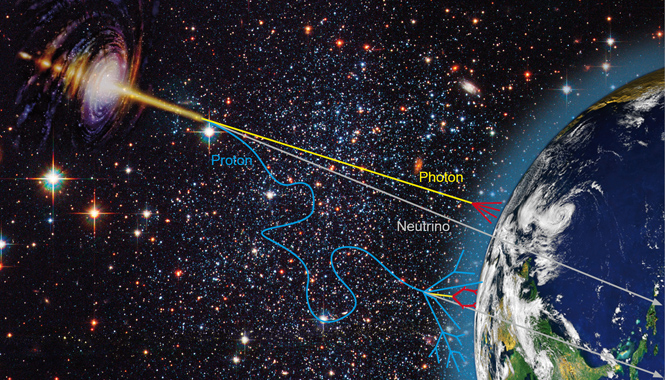
\includegraphics[width=0.9\textwidth]{images/astro-web-titel.jpg}
	\caption{Visualization of the behaviors of different messengers
		particles in modern astronomy.
		Photons and neutrinos travel the universe without deflection,
		because they do not carry an electric charge.
		Neutrinos interact less than photons both in the universe and in the detector,
		which leads to a high proportion passing through earth.
		Charged cosmic rays get deflected by interstellar
		magnetic fields and thus generally do not allow for a assignment to a cosmological source.
		This illustration lacks gravitational waves 
		as these have only recently been measured.
		The image is taken from the DESY-website at \cite{desy_mm_astro}.
	}
	\label{fig:multi_messenger}
\end{figure}


\subsection{Charged Cosmic Rays}
The term charged cosmic rays summates all types of charged particles from
extra terrestrial sources with the main proportion being protons
\cite{Dembinski:2017zsh}.


\begin{figure}
	\centering
	\captionsetup{width=0.9\linewidth}
	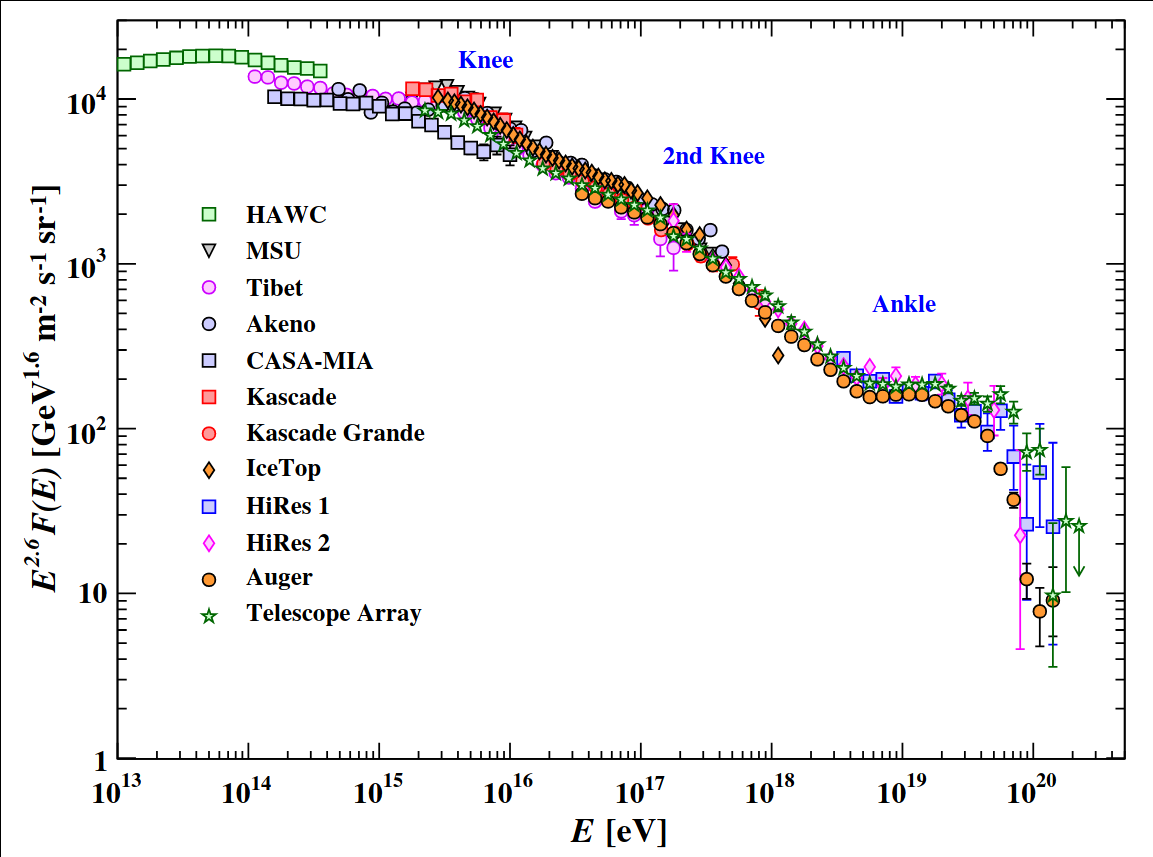
\includegraphics[width=0.9\textwidth]{images/cr_spectrum.png}
	\caption{Combined plot of the all-particle cosmic ray spectrum,
		measured by various air shower experiments in different
		energy ranges. One can see the two "knees" where
		the spectrum gets steeper and the "ankle" at high
		energies where the spectrum seems to get flatter again.
		At the very highest energies the measurements point towards
		a rapid decrease in flux.
		The image is taken from the current review of particle physics
		by the particle data group \cite{pdg19}.
	}
	\label{fig:cr_spectrum}
\end{figure}

Figure \ref{fig:cr_spectrum} shows the flux of charged cosmic rays over 
many orders of magnitude in energy which mainly follows 
a power law $E^{-\gamma}$ with $\gamma$ somewhere between 
2.7 and 3.3. Deviations from this crude approximation are 
usually referred to as the first and second knee and the ankle 
at $\num{5e15}, \num{2e17}$ and $\SI{5e18}{\electronvolt}$ respectively,
with the second knee being less researched and of less importance
to most models.

The (first) knee could be explained by the assumption that the galactic sources
reach their maximum energy at around that energy and the higher energy rays
are mostly produced by extragalactical sources \cite{pdg19}.
Other explanations assume the knee to not be an intrinsic property of the acceleration process,
but to form during the propagation either thoughout the galaxy or
inside the atmosphere (For a more detailed look at different 
theoretical models have a look
at \cite{HORANDEL2004241}).

At the very highest energies, the flux seems to rapidly decrease,
which may point towards a maximum energy
that cosmological sources can produce or towards destructive interaction with 
the cosmic microwave background \cite{bookap}.

\iffalse

The current model assumes the high energy cosmic rays to be produced 
mainly in supernova remnants (SNRs) through the expanding shock waves \cite{bookap}.
Our following overview closely follows the notation from \cite{bookap}, for more details
about DSA the reader is referred to \cite{gaisser_engel_resconi_2016} and
\cite{drury1983introduction}.

An important description of the acceleration process has been
worked out by Enrico Fermi in 1949 \cite{PhysRev.75.1169}.
The main assumption is that the charged particle performs 
stochastic scattering with a (partially ionized) moving gas cloud.
Because the gas cloud has a much higher effective mass than the particle and
includes non constant magnetic fields, it acts as magnetic mirrors.
The particle would gain energy with each scattering until it breaks free from the 
gas cloud. This is nowadays referenced to as the second-order Fermi mechanism, 
because the energy gain is proportional to $\beta^2$, with $\beta$
the velocity of the gas cloud and $\beta \ll 1$.

This however is not enough to accelerate particles to the observed energies.
An acceleration linear in $\beta$ can be explained through a model called
Diffuse Schock Acceleration (DSA), also referenced as first-order
Fermi mechanism.

This requires a gas cloud where the gas directions are highly correlated,
which is the case in SNRs.

With the shock wave rapidly moving, one can divide the surrounding gas in 
an upstream and downstream component. In the reference frame of the shock
the upstream component runs into the shock with 
velocity $u_u$ and the downstream component moves away from 
it with velocity $u_d$.
A particle in the upstream region would then experience reflection on 
magnetic mirrors similar as in the second-order case, but because of the 
moving shock front the velocity changes happen mostly 
parallel to the direction of the shock movement.
These collisions between parallel magnetic mirrors mostly
invert the direction of the particle each time, every collision pair 
is referenced to as a bound-rebound cycle with an energy gain of 

\begin{equation}
	\langle \frac{\Delta E}{E} \rangle 
	\simeq -2\beta \langle \cos{\theta} \rangle
	\simeq \frac{4}{3}\beta
	\equiv \epsilon
\end{equation}

with the scattering angle $\theta$.
Because this energy gain is very much constant in the particles energy,
a particle could reach very high 
energies only limited by the number of bound-rebound cycles $n$.
On the other hand higher particle energy $E$ (and thus speed), 
comes with a higher probability of escaping the shock region, denoted 
as $P_{E_n}$. This restricts the number of cycles and makes 
higher particle energies less likely.

The first-order Fermi mechanism leads to a exponential energy spectrum 
\begin{equation}
	\frac{dN}{dE} \propto \left(\frac{E}{E_0}\right)^{-\Gamma}
\end{equation}

with$\Gamma \approx 2$.
This primary energy spectrum gets modified further during the particles 
journey from the galactic sources to the earth.
Since particles with a higher energy have a higher probability to escape 
from the Galaxy, the spectrum gets steeper:
\begin{equation}
	\frac{dN}{dE} \propto \left(\frac{E}{E_0}\right)^{-\Gamma-\delta}
\end{equation}

Predictions for $\delta$ are highly model dependent, with \cite{bookap}
stating $\delta$ to be in the range $0.3-0.6$ and \cite{refId0}
finding values of \num{0.234} and \num{0.86}, depending on the model.

With this model, energies up to the first ankle can be explained.
Higher energy particles are sometimes assumed to be of extragalactical origin
\cite{Baring:1997ka}.

Cosmic rays get researched by a lot of different experiments,
also with IACTs. 
(Hier mehr schreiben?)

\fi

\subsection{Gamma Radiation}
In contrast to charged cosmic rays, $\gamma$-particles point towards
their sources, allowing to search for sources of radiation.
In general $\gamma$-radiation refers to photons at all wavelength,
the term $\gamma$-rays in contrast is assigned to the very 
highest energy particles with energies above those of X-rays.
A schematic illustration of the different photon wavelengths
can be seen in figure \ref{fig:em_spectrum}.

\begin{figure}
	\centering
	\captionsetup{width=0.9\linewidth}
	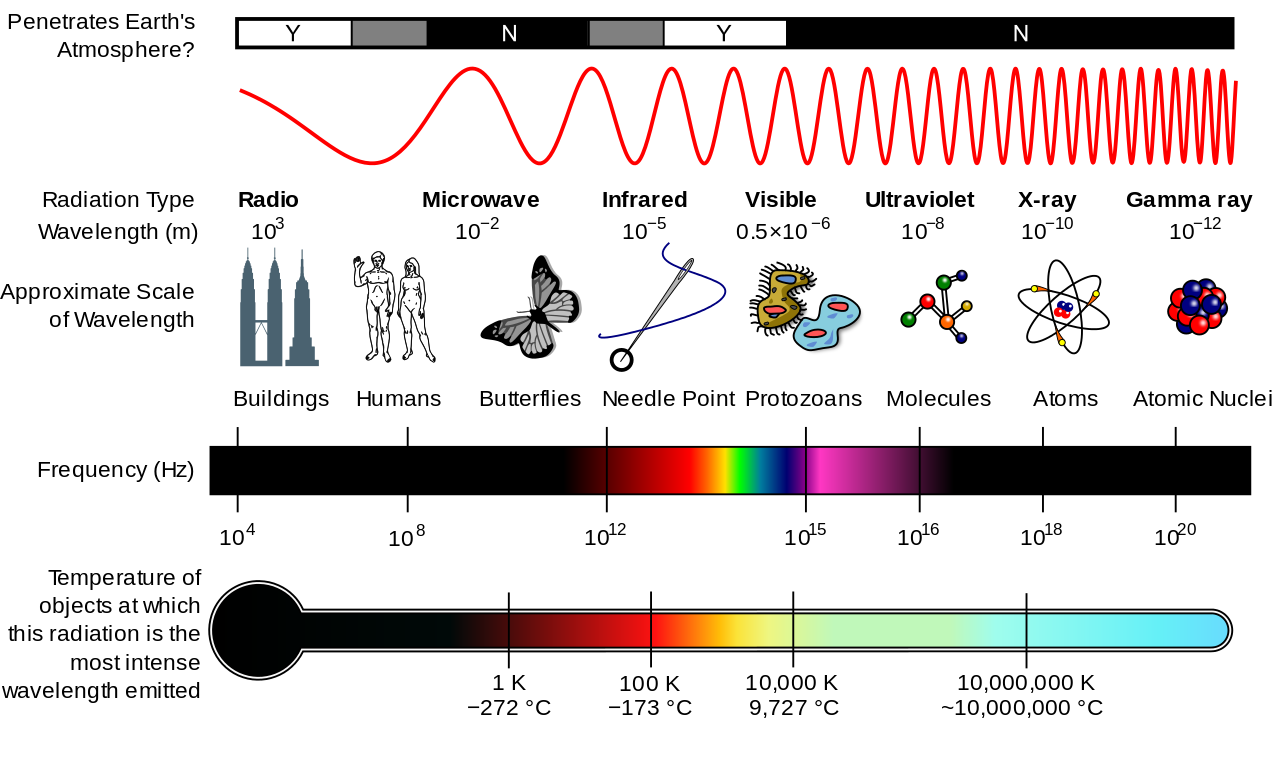
\includegraphics[width=.9\textwidth]{images/em_spectrum.png}
	\caption{An overview of properties and applications of photons
		on a wide range of wavelengths.
		Radio-photons possess very low energies, gamma-rays 
		carry the very highest energies.
		Visible light lies in between, technical 
		applications exist for all the shown wavelengths.
		As indicated by the temperature bar at the bottom,
		$\gamma$-rays can not feasibly be produced by thermal radiation.
		The image is taken from \cite{wiki_em}.}
	\label{fig:em_spectrum}
\end{figure}

\iffalse

Creation of high-energy gamma-rays is due to a lot of 
different processes. Among these we want to give a brief 
overview of two important processes, focusing on 
photon emission from an initial pure electron distribution.
Depending on the studied case other emission factors 
might play important roles as well, such as 
the $\gamma$-production from $\pi^0$-decays in cosmic rays.

\textbf{Synchroton Radiation}

Sources of cosmic and gamma rays often times include 
high magnetic fields. Any moving charged particle will thus be
deflected perpendicular to its moving direction
due to the Lorentz-force, forcing them on a radial trajectory.
At the same time a relativistic charged particle, 
that gets accelerated radially, emits synchroton 
photons with average energy given by 
equation \ref{eq:synchroton}

\begin{equation}
	\langle E_{\gamma} \rangle \propto \frac{1}{M_P} E_P^2 B^2.
	\label{eq:synchroton}
\end{equation}

Hereby $M_P$ and $E_P$ denote the accelerated particle's 
mass and energy respectively. With the inverse mass dependency 
it is immediately evident that 
synchroton radiation plays a major role in leptonic 
emission and much less in hadronic emission.

It is important to remember that this affects the 
initial electron distribution, by reducing the electrons energy.
This is sometimes referred to as synchroton cooling.

The emitted synchroton spectrum needs to be further modified 
if the emitting region is optically thick and photons 
get absorbed by the medium.
This is always true for our cases, as the regions contains 
both magnetic fields and a high density of electrons.

\textbf{(Inverse) Compton Scattering}
In a classical particle interpretation photons and electrons 
can collide exchanging energy and altering their directions.
For the normal case of Compton scattering the electron 
is assumed to be at rest and the photon can never gain 
energy by scattering of the electron.
This can be 
seen by the increase in wavelength in equation \ref{eq:compton},
with $\lambda^{\prime}$ denoting the the scattered photons 
wavelength, $\lambda$ denoting the initial photons wavelength  
and $\Theta$ the scattering angle.

\begin{equation}
	\lambda^{\prime} - \lambda  \propto \left(1-\cos{\Theta} \right)
	\label{eq:compton}
\end{equation}


If the electron itself is moving with much higher energy
than the photon, this changes and the photon can gain substantial energy.
This is referenced as inverse Compton scattering.
In that case transforming the equations to the 
electron's frame of reference and back to the labor frame 
boosts the photons energy by a factor $\gamma$ for each transformation, 
with $\gamma$ being the Lorentz factor of the electron.

A limit to the photon energies is set by the scattering cross
section, which reduces with higher photon energies.
For low energies the cross section can be approximated by 
the Thomson cross section, for high energies
one uses the Klein-Nishina cross section.

The Synchroton Self Compton model combines the above mentioned
effects to produce a photon energy distribution from an
electron distribution, which is often times assumed to
follow a power-law spectrum initially.
The free parameters of the model can be interpreted as 
three frequencies: The minimum injection frequency $\nu_m$, 
the cooling frequency $\nu_c$ and the self-absorption frequency $\nu_a$.
Depending on the order of these parameters, different 
photon distributions can be generated.

For more general information about the generation of photon 
and cosmic ray spectra, the reader is referred to 
\cite{gaisser_engel_resconi_2016}
or
\cite{bookap}.

For a detailed analysis of the influence of the parameters of
the Synchroton Self Compton model, 
the lecture of \cite{10.1093/mnras/stt1461} is advised.


Emitted $\gamma$-rays can be observed either directly
from outside the atmosphere via satellites or indirectly
via ground based gamma astronomy. In the later case
IACTs are used to detect electromagnetic showers induced
by the collision of high energy photons with particles in the atmosphere.
% An example for direct observation could be the Fermi 
% Gamma-Ray Space Telescope \cite{Atwood_2009},
% an example for ground based observation could be the
% MAGIC-experiment \cite{LORENZ2004339}.
\fi

\iffalse
\subsection{Neutrinos}
Even less affected by interactions on the way 
from the source to the earth are neutrinos ($\nu$).
Due to their small interaction cross sections and no electric charge, they 
suffer very little from absorption or deflection.
For very much the same reasons detecting neutrinos is much harder
than detecting photons or charged particles.

The small cross section requires to build huge detectors, 
the ICECUBE having a detector volume of \SI{1}{\kilo\meter^3}
\cite{Abbasi:2008aa}.
An illustration of the ICECUBE Neutrino Observatory
is shown in figure \ref{fig:icecube}.
\begin{figure}
	\centering
	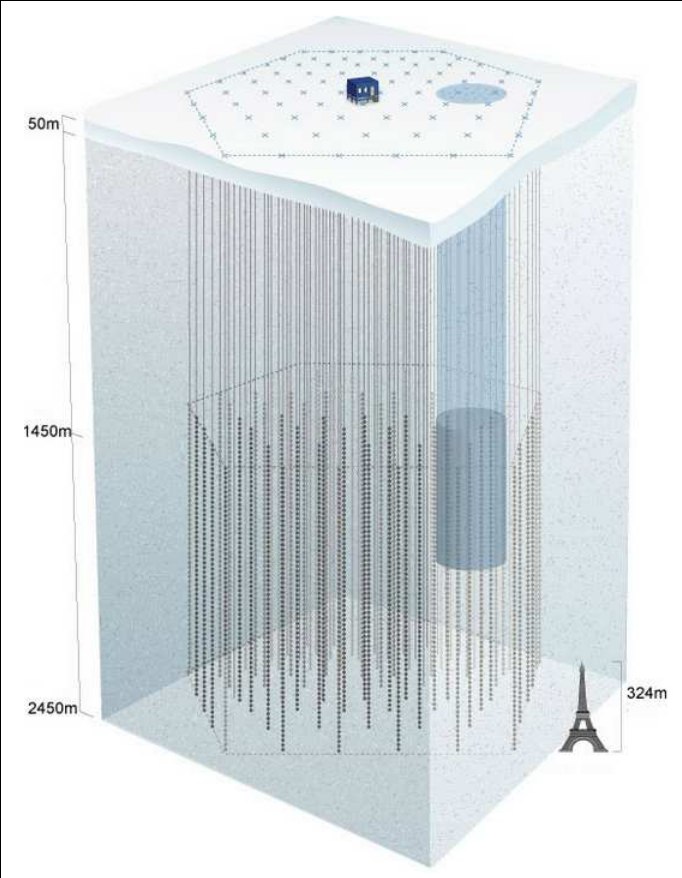
\includegraphics[width=0.8\textwidth]{images/icecube.png}
	\caption{icecube illustration, cite that \cite{Abbasi:2008aa}}
	\label{fig:icecube}
\endrvation.
They are a direct result from general relativity and occur
at certain constellations of very high masses, such as 
merging black holes.

An illustration of such an event is shown in figure \ref{fig:gravi_waves}. 
\begin{figure}
	\centering
	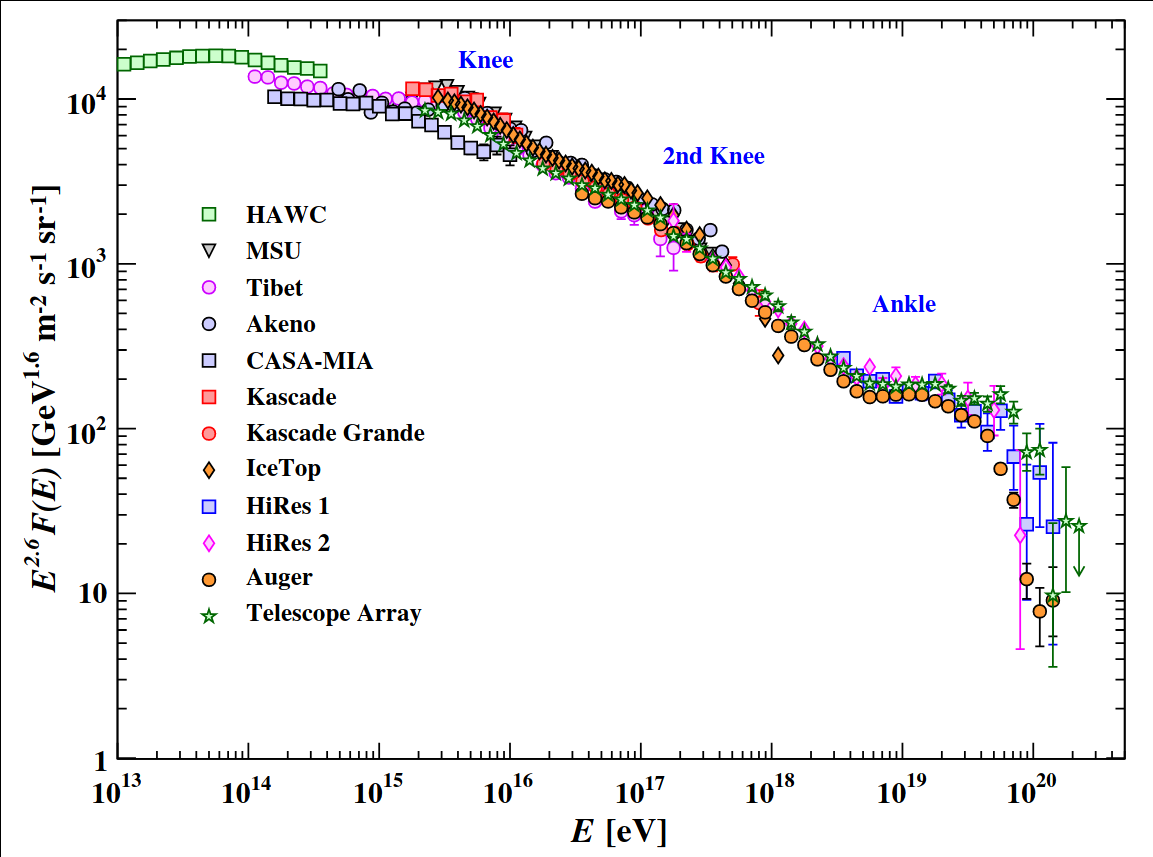
\includegraphics[width=0.8\textwidth]{images/cr_spectrum.png}
	\caption{images}
	\label{fig:gravi_waves}
\end{figure}


We can detect them using large size interferometers such as
the LiGO's three detectors (citation needed).
\fi

\section{Detection of Gamma Rays with Ground Based Telescopes}
The primary particles of gamma or cosmic rays cannot be 
observed with IACTs directly. Instead one can measure the secondary particles
that emerge from the particles interaction with matter.

If the primary particle energy is high enough, the resulting 
secondary
particles can interact with the atmosphere themself, thus starting a 
cascade of secondary particles.

Depending on whether the primary particle is 
a photon/electron/positron or a heavier particle such as a proton 
or iron core, the interactions vary.

This leads to a separation of electromagnetic and hadronic showers.
If the experiment is primarly looking for 
gamma rays, e.g. if measuring a known source like the Crab Nebula, 
the hadronic showers act as dominant background.
As hadronic showers get observed much more frequently, 
the identification of the primary particle type is a very important 
task, often times referred to as gamma-/hadron-separation.

To understand how these showers differ, we will have a very brief look
at the relevant interactions at the primary particle energies
we want to observe.

\subsection{Electromagnetic Showers}
Electromagnetic showers consist mainly of three types of particles:
\begin{enumerate}
	\item{Photons $\gamma$}
	\item{Electrons $e^-$}
	\item{Positrons $e^+$}
\end{enumerate}

The main interaction for high energy photons is pair 
production, generating an $e^+/e^--$pair where the energy of 
the secondary particles equals the photon energy.
On the other hand high energy electrons (and positrons) lose 
most of their energy by radiation, leading to a photon with 
an energy close to the electron energy.
Only at lower particle energies other interaction forms show their impact,
with particle scattering and ionization 
leading to more continuous energy losses.

These assumptions lead to the most basic model of an 
electromagnetic shower, proposed by Bhabha and Heitler in 1937
\cite{doi:10.1098/rspa.1937.0082}.
It starts with a high energy primary photon before its interaction in the atmosphere 
(The original paper starts from a high energy electron interacting in lead actually.
As will be evident this does not concern our qualitative look at the model.) and continues 
the calculation in discrete epochs.
The photon produces a pair of $e^-$ and $e^+$ in the first epoch.
Because of the high energies at play, the direction of these secondary 
particles does not deviate significantly from the photons direction, 
making the problem essentially one-dimensional.
The $e^+/e^-$ continue on to radiate a photon each and the cycle continues.
Each step doubles the number of particles in the shower with each particle 
on average getting half the energy of its parent particle.
These processes continue until the energy of the $e^+/e^-$ becomes low enough for
continuous ionization processes to become relevant.
At this point the particle is considered to be stopped and the shower
does not evolve further.

Today Monte Carlo calculations get used to simulate the properties 
of particle showers in the atmosphere.
The most common software to model the atmospheric interactions is
CORSIKA \cite{Engel:2018akg}.

Figure \ref{fig:gamma_shower} illustrates the Bhabha-Heitler model (left)
and a \SI{100}{\giga\electronvolt} gamma shower, simulated with CORSIKA (right).

\begin{figure}
	\centering
	\captionsetup{width=0.9\linewidth}
	\begin{subfigure}{.7\textwidth}
  		\centering
  		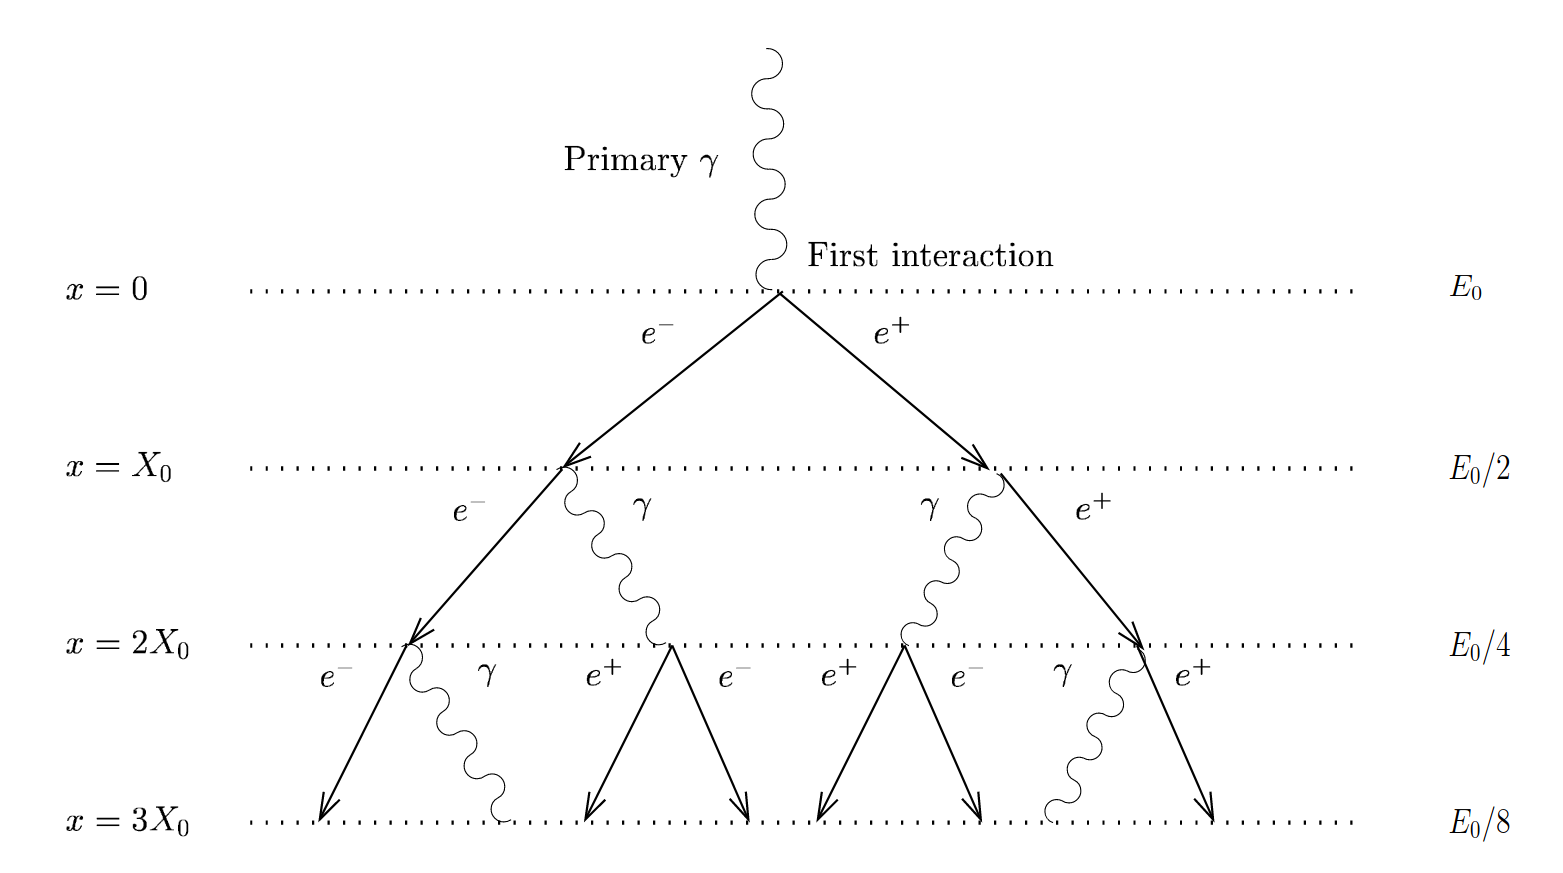
\includegraphics[width=\linewidth]{images/em_shower_illustration.png}
	\end{subfigure}%
	\begin{subfigure}{.2\textwidth}
 		\centering
		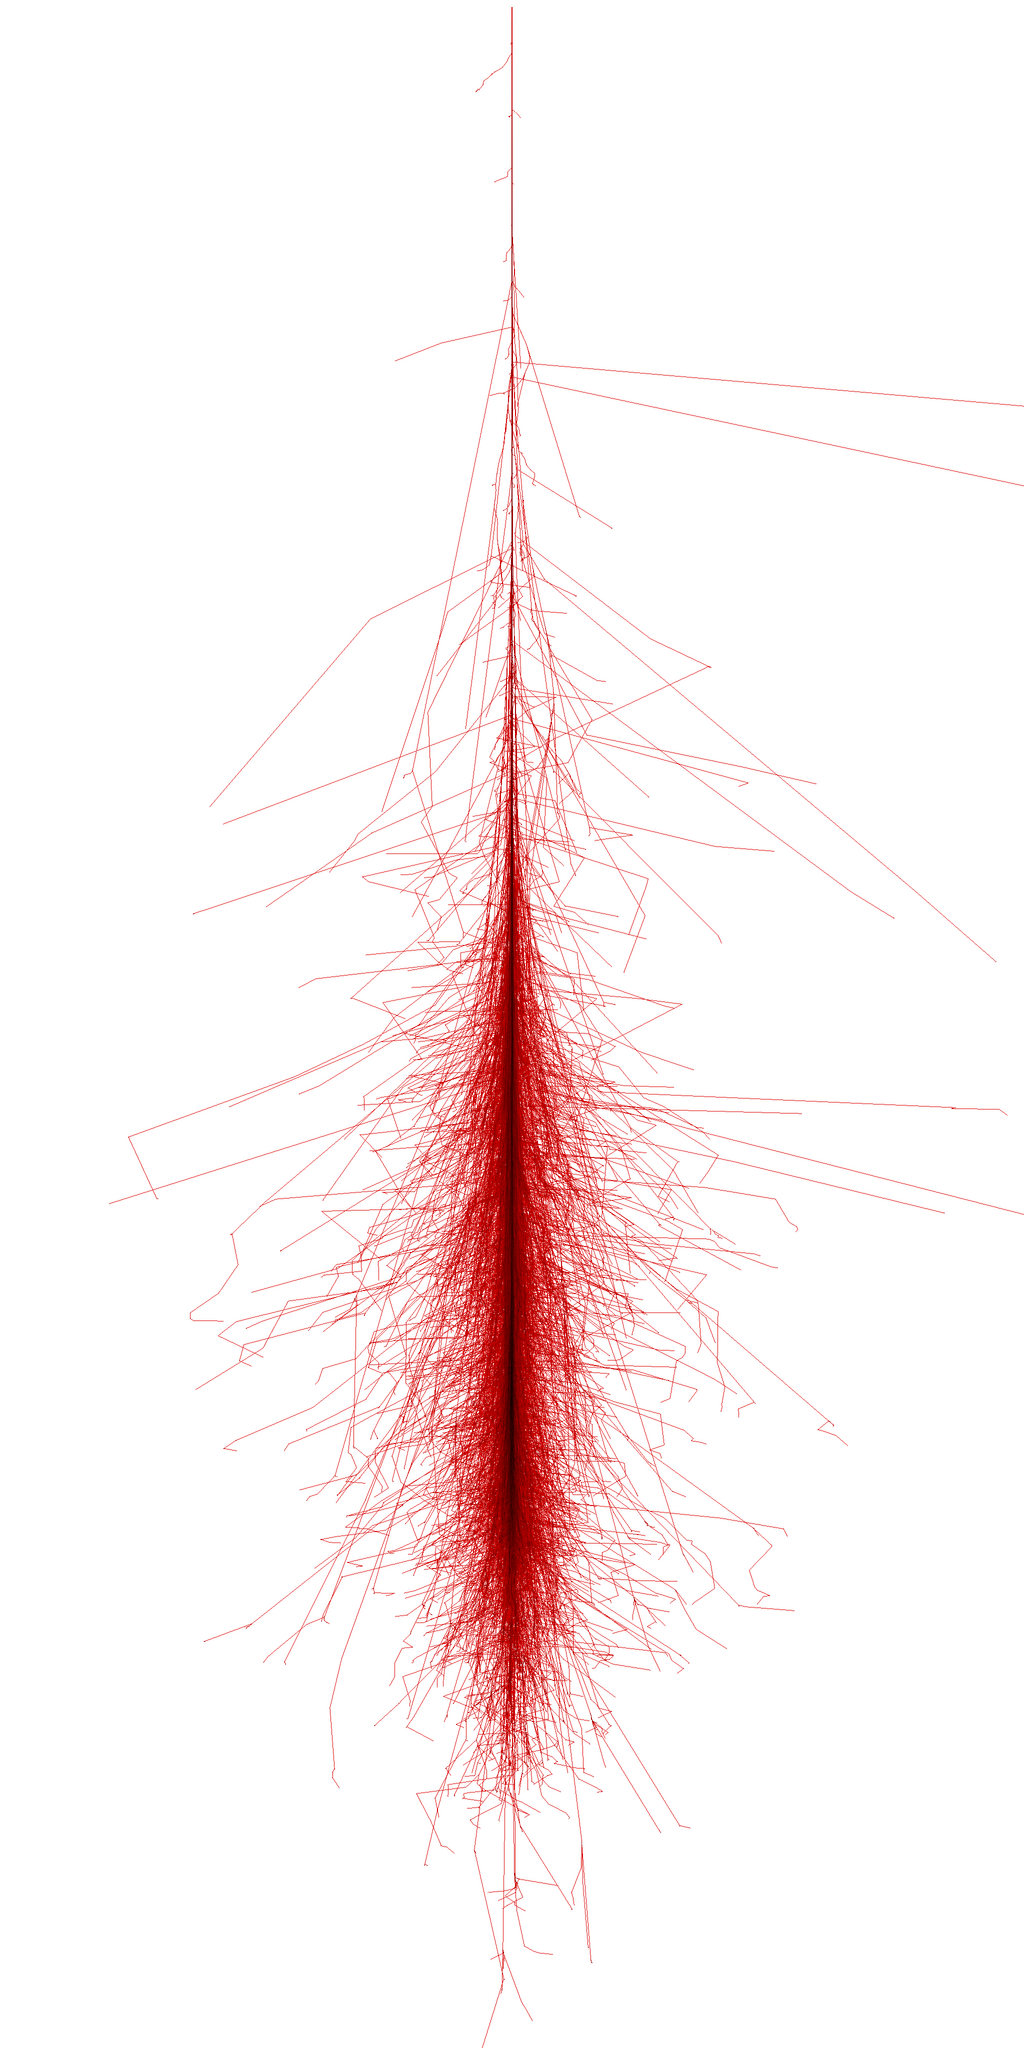
\includegraphics[width=\linewidth]{images/corsika_100gev_photon.png}
	\end{subfigure}
	\caption{Schematic illustration and simulation of a $\gamma$ air shower. \\
		Left: A schematic illustration of the first epochs of the 
		Bethe-Heitler shower model with equal radiation lengths for
		bremsstrahlung and pair production.
		The image is taken from an inaugural thesis 
		by Stefan Funk \cite{funk_doctor}. \\
		Right: A \SI{100}{\giga\electronvolt} gamma-shower as xz-projection, simulated with CORSIKA.
		The shower is relatively contained with only little extent perpendicular 
		to the shower direction (z-axis). The image is taken from 
		the CORSIKA-website \cite{corsika_showers}}
	\label{fig:gamma_shower}
\end{figure}

\subsection{Hadronic Showers}
Hadronic shower include all the interactions known from 
electromagnetic showers, but add nuclear interactions on top.
These lead to non-negligible additional energy losses 
and the creation of secondary hadronic particles.

Approximations are more difficult to do and monte carlo simulations 
become the only way to reasonably calculate shower behavior.

At the end of the shower a relevant portion of the particles have decayed into the 
lightest hadronic particles, pions ($\pi^0, \pi^+, \pi^-$), of which the neutral pions 
rapidly decay into photons.
This means that a part of the hadronic shower
eventually becomes an electromagnetic subshower.

Figures \ref{fig:proton_shower}
shows some of the particles generated in a hadronic shower (left)
and a \SI{100}{\giga\electronvolt} proton shower, simulated with CORSIKA (right).

\begin{figure}
	\centering
	\captionsetup{width=0.9\linewidth}
	\begin{subfigure}{.7\textwidth}
  		\centering
  		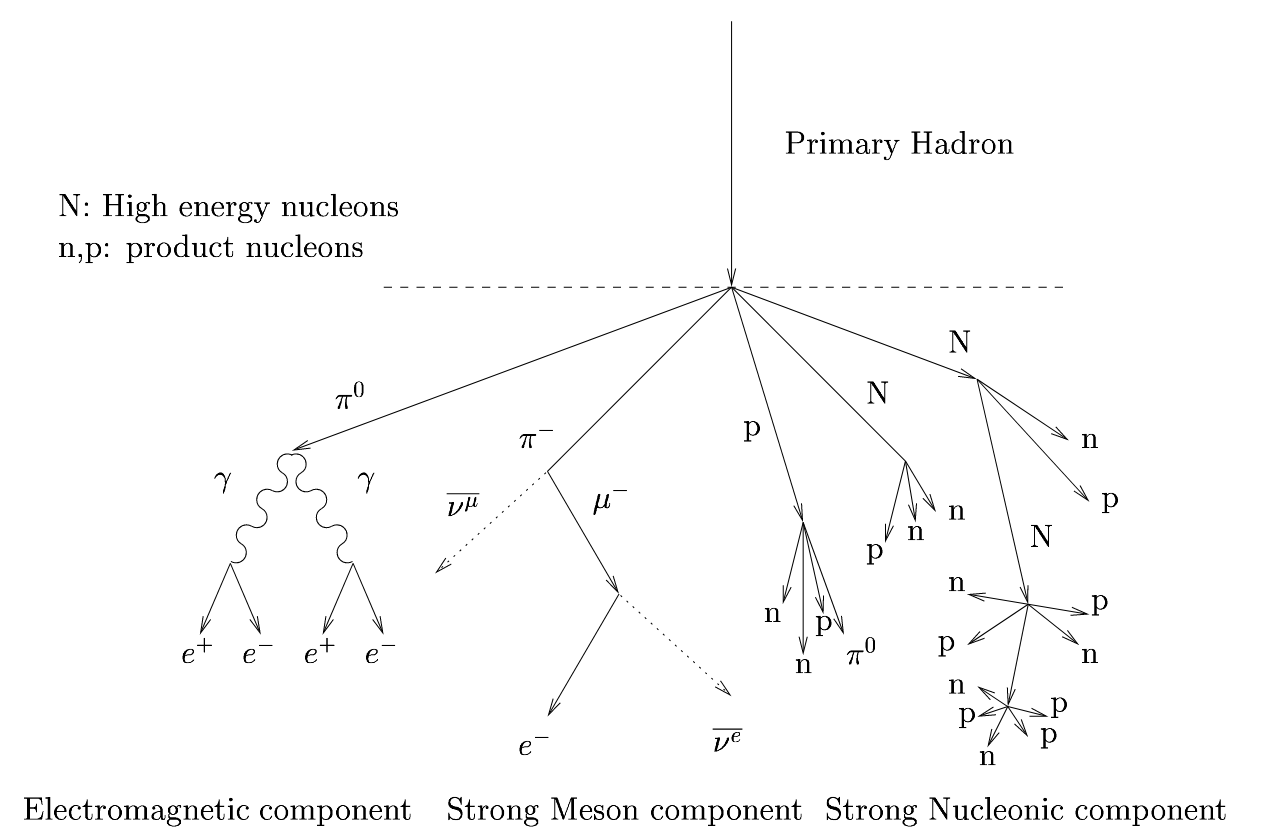
\includegraphics[width=\linewidth]{images/hadron_shower_illustration.png}
	\end{subfigure}%
	\begin{subfigure}{.2\textwidth}
 		\centering
		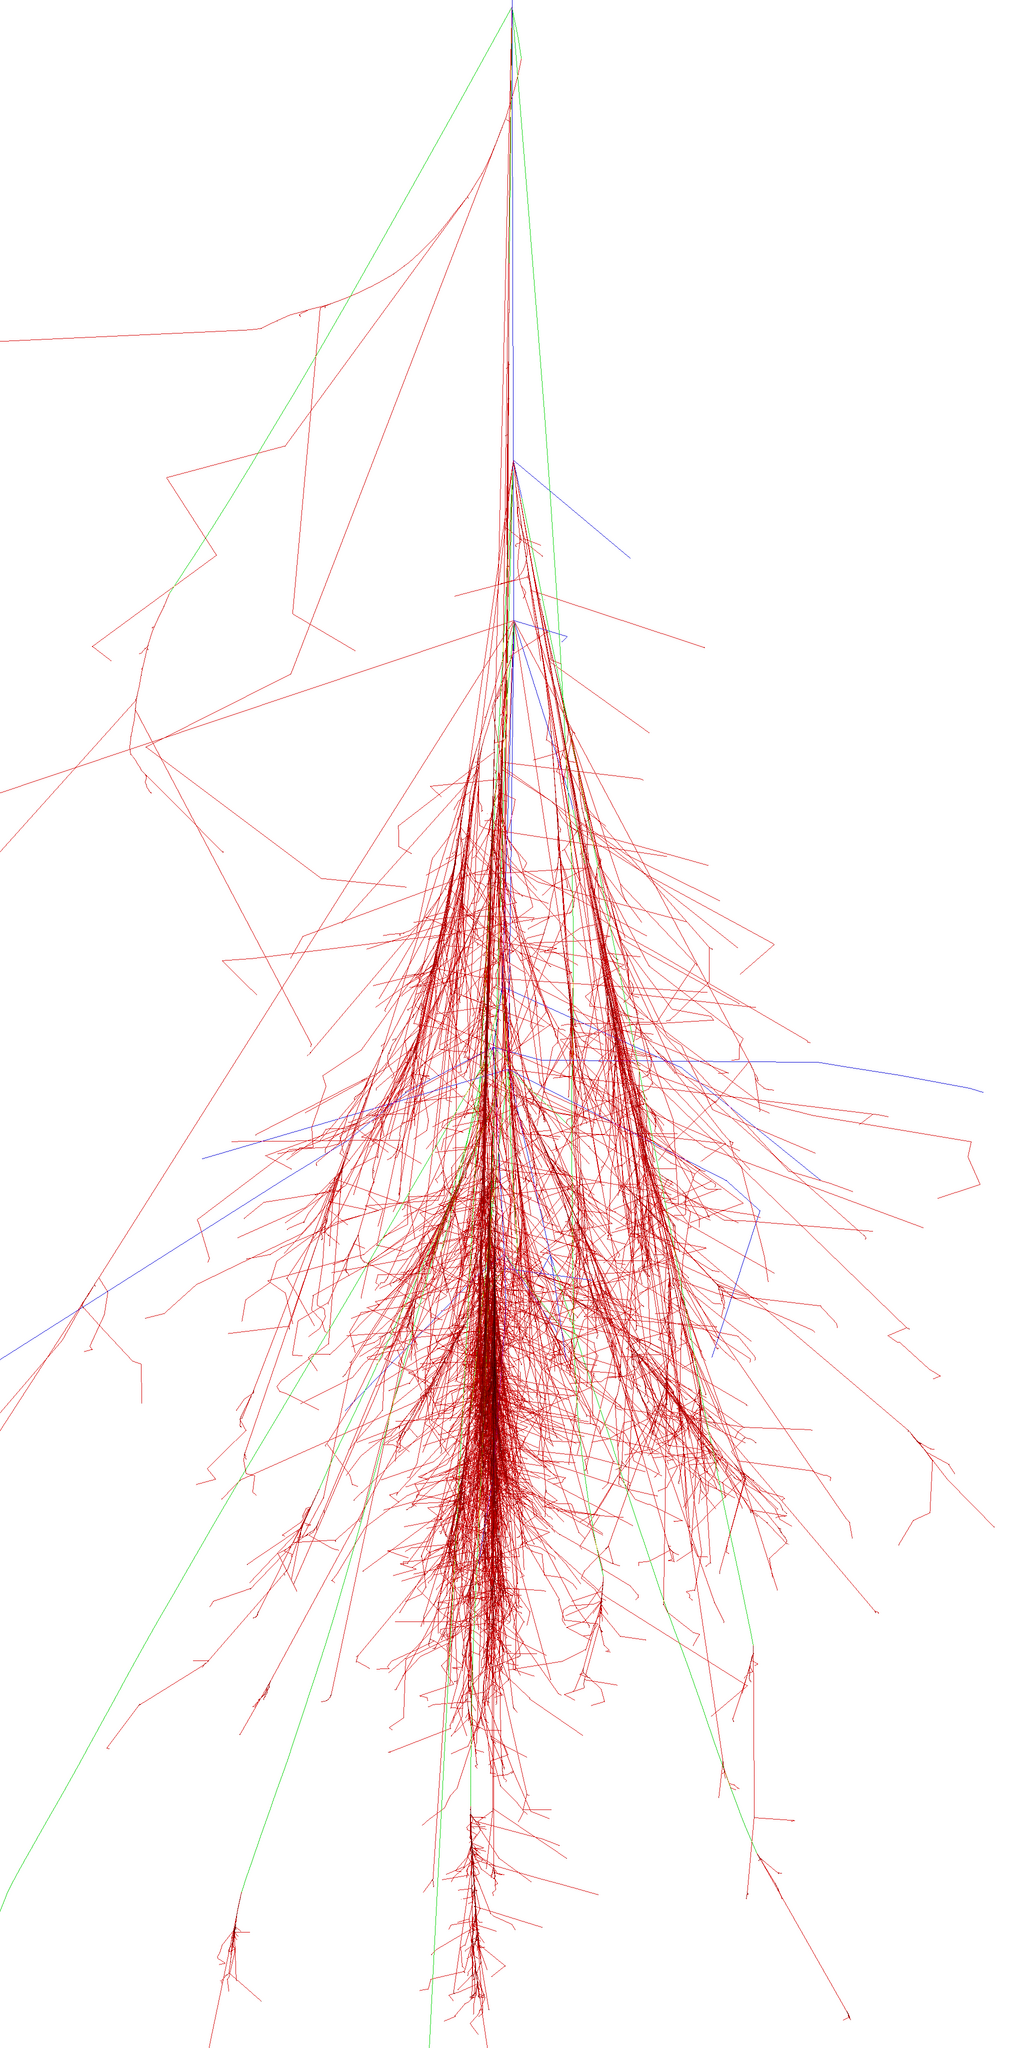
\includegraphics[width=\linewidth]{images/corsika_100gev_proton.png}
	\end{subfigure}
	\caption{Schematic illustration and simulation of a proton air shower.\\
		Left: A purely qualitative,
		schematic illustration of the generation of a hadronic shower.
		It shows how the primary hadron generates different subshowers
		with vastly different particles.
		The image is taken from an inaugural thesis 
		by Stefan Funk \cite{funk_doctor}.\\
		Right: A \SI{100}{\giga\electronvolt} proton-shower as xz-projection,
		simulated with CORSIKA.
		The shower is less contained than the gamma shower of equal energy in 
		figure \ref{fig:gamma_shower}.
		Different colors indicate different particle types.
		The image is taken from 
		the CORSIKA-website \cite{corsika_showers}.}
	\label{fig:proton_shower}
\end{figure}

\subsection{Measuring Events}
\label{sec:measuring}

The way IACTs detect particle showers in the atmosphere is by their emittance 
of Cherenkov light. Cherenkov light gets emitted whenever a 
charged particle moves through a dielectric medium with a velocity 
exceeding the local speed of light, which happens in air for the
highly relativistic particles we are lokking at.

Cherenkov photons get collected by the mirror(s) of a telescope
and projected onto a camera system mounted above the mirror.
With this setup IACTs usually reach a field of view of a few degree.
Figure \ref{fig:iact_mirror_camera} illustrates this setup.

\begin{figure}
	\centering
	\captionsetup{width=0.9\linewidth}
	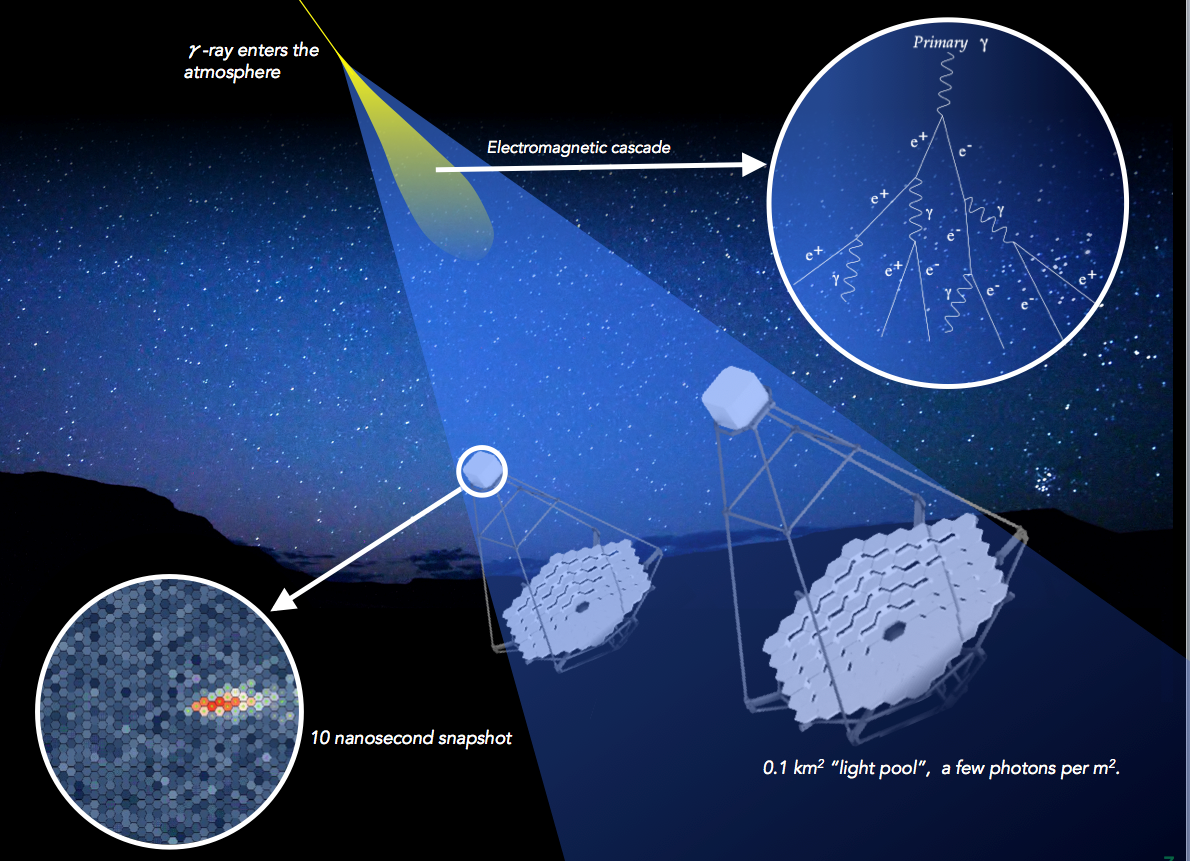
\includegraphics[width=0.9\textwidth]{images/cta47.png}
	\caption{A schematic illustration of the working principles of 
	an IACT experiment:
	A $\gamma$-ray produces an air shower in the atmosphere
	that points roughly towards the telescopes.
	Cherenkov light from the air shower 
	hits the mirrors and gets focused into a camera mounted on top.
	An illustration of the resulting image after integrating 
	\SI{10}{\nano\second} of the pixel measurements
	can be seen in the left bottom corner.
	The image is taken from the official CTA-website \cite{cta_web}.}
	\label{fig:iact_mirror_camera}
\end{figure}


Upon detection of a shower and performing the low-level analysis,
the usual tasks of a high-level analysis include reconstructing 
three key properties of the primary particle:
\begin{enumerate}
	\item{Shower type (e.g. gamma or hadronic)}
	\item{Primary particle energy}
	\item{Shower direction/source position}
\end{enumerate}

In most cases the reconstruction can be improved heavily by cleaning the image first.
Figure \ref{fig:shower_cleaning} shows a simulated $\gamma$-induced shower image
in the camera of the Large Sized Telescope (LST, see section \ref{sec:lst} for more details of the telescope)
before and after cleaning.

\begin{figure}
	\centering
	\captionsetup{width=0.9\linewidth}
	\begin{subfigure}{.45\textwidth}
  		\centering
  		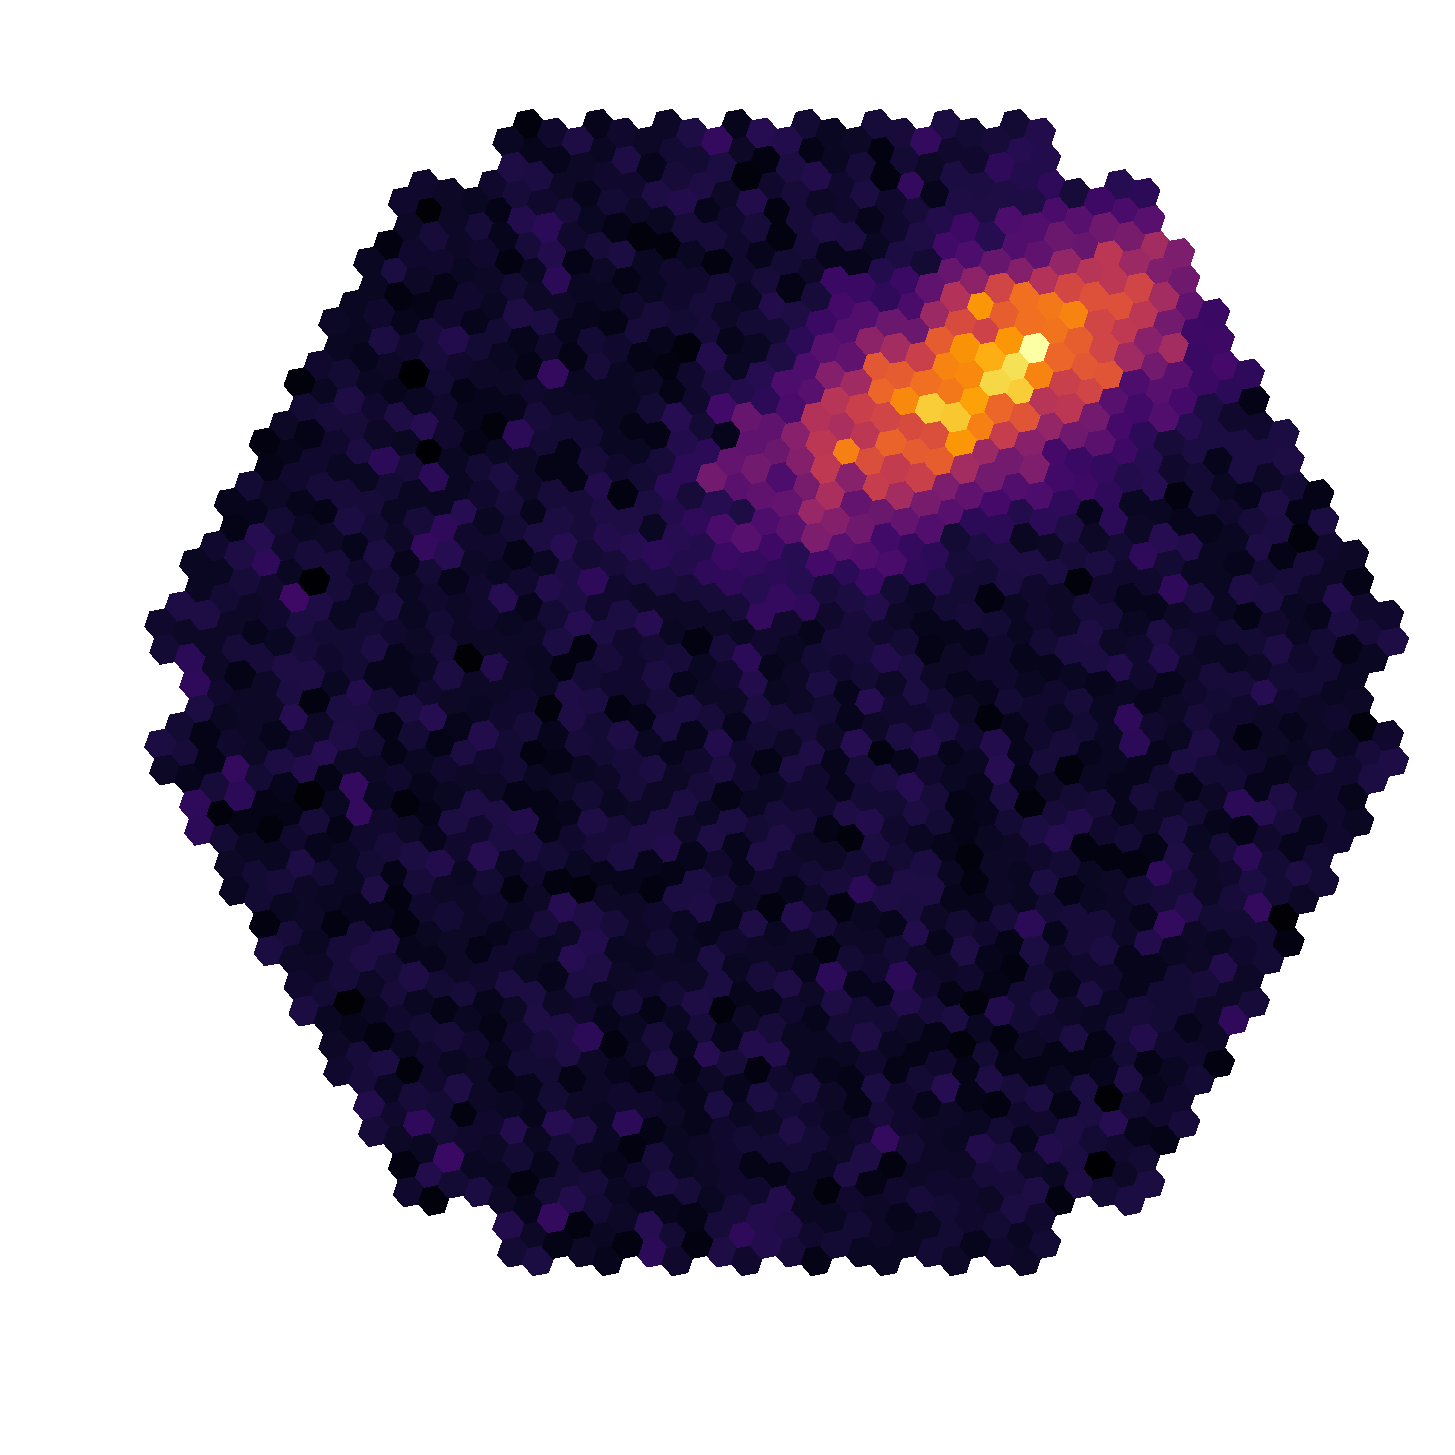
\includegraphics[width=\linewidth]{Plots/hillas_raw.pdf}
	\end{subfigure}%
	\begin{subfigure}{.45\textwidth}
 		\centering
		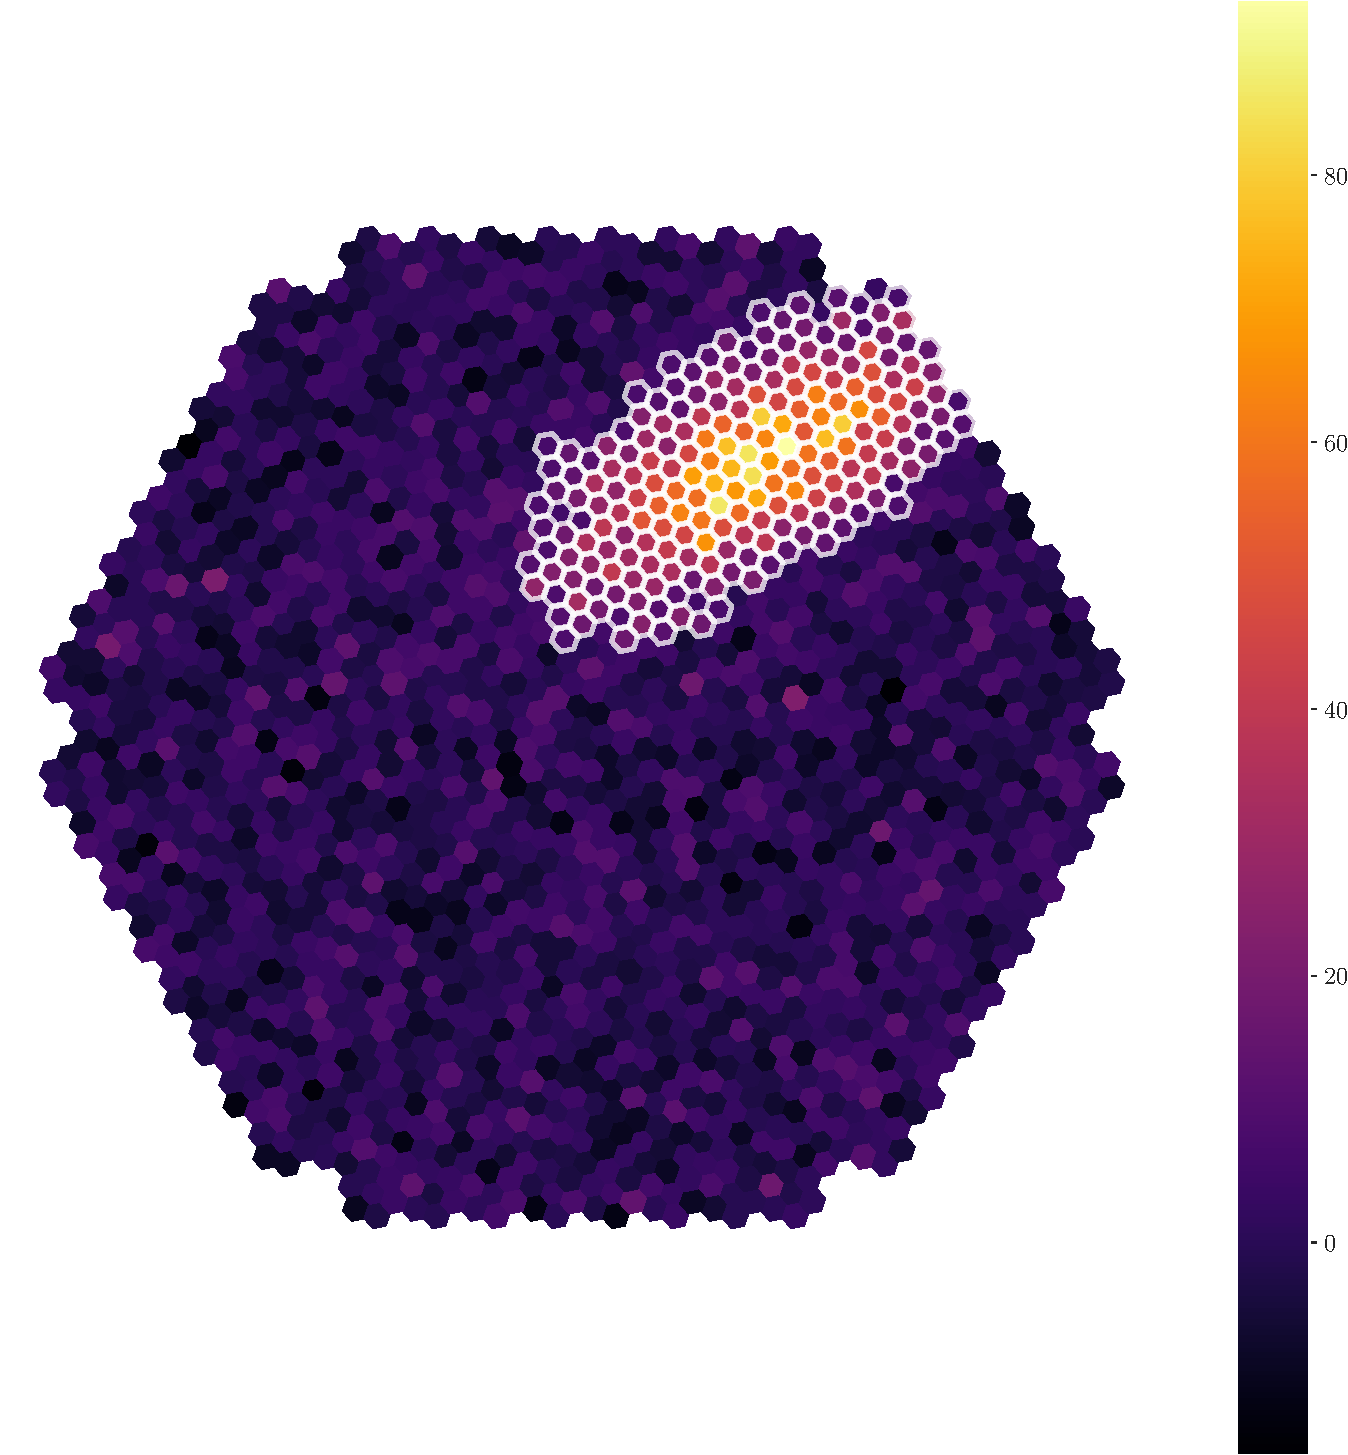
\includegraphics[width=\linewidth]{Plots/hillas_cleaned.pdf}
	\end{subfigure}
	\caption{An idealized gamma-shower in the camera of a LST
	    before and after cleaning.
		The pixel colors show the intensity as integrated 
		waveform in each pixel. 
		Brighter color indicates higher intensity.\\
		Left: The signal directly after
		the waveform integration. Non-signal pixels are noisy. 
		Right: Image after the cleaning-algorithm has been 
		applied. The noise in the non-signal pixels is gone,
		improving the analysis.}
	\label{fig:shower_cleaning}
\end{figure}

The analysis then usually involves describing the 
shower image as an ellipse and calculating the so called hillas parameters,
allowing the description of the shower image with only a handful of parameters.
The historical approach can be read up in 
a famous paper of A.M. Hillas \cite{hillas_params}.

An illustration with the hillas ellipse on top of the shower image 
can be seen in figure \ref{fig:hillas_params}.
This also includes an estimate of the true source position with the DISP-method
which we will use and explain at later stages.

\begin{figure}
	\centering	
	\captionsetup{width=0.9\linewidth}
	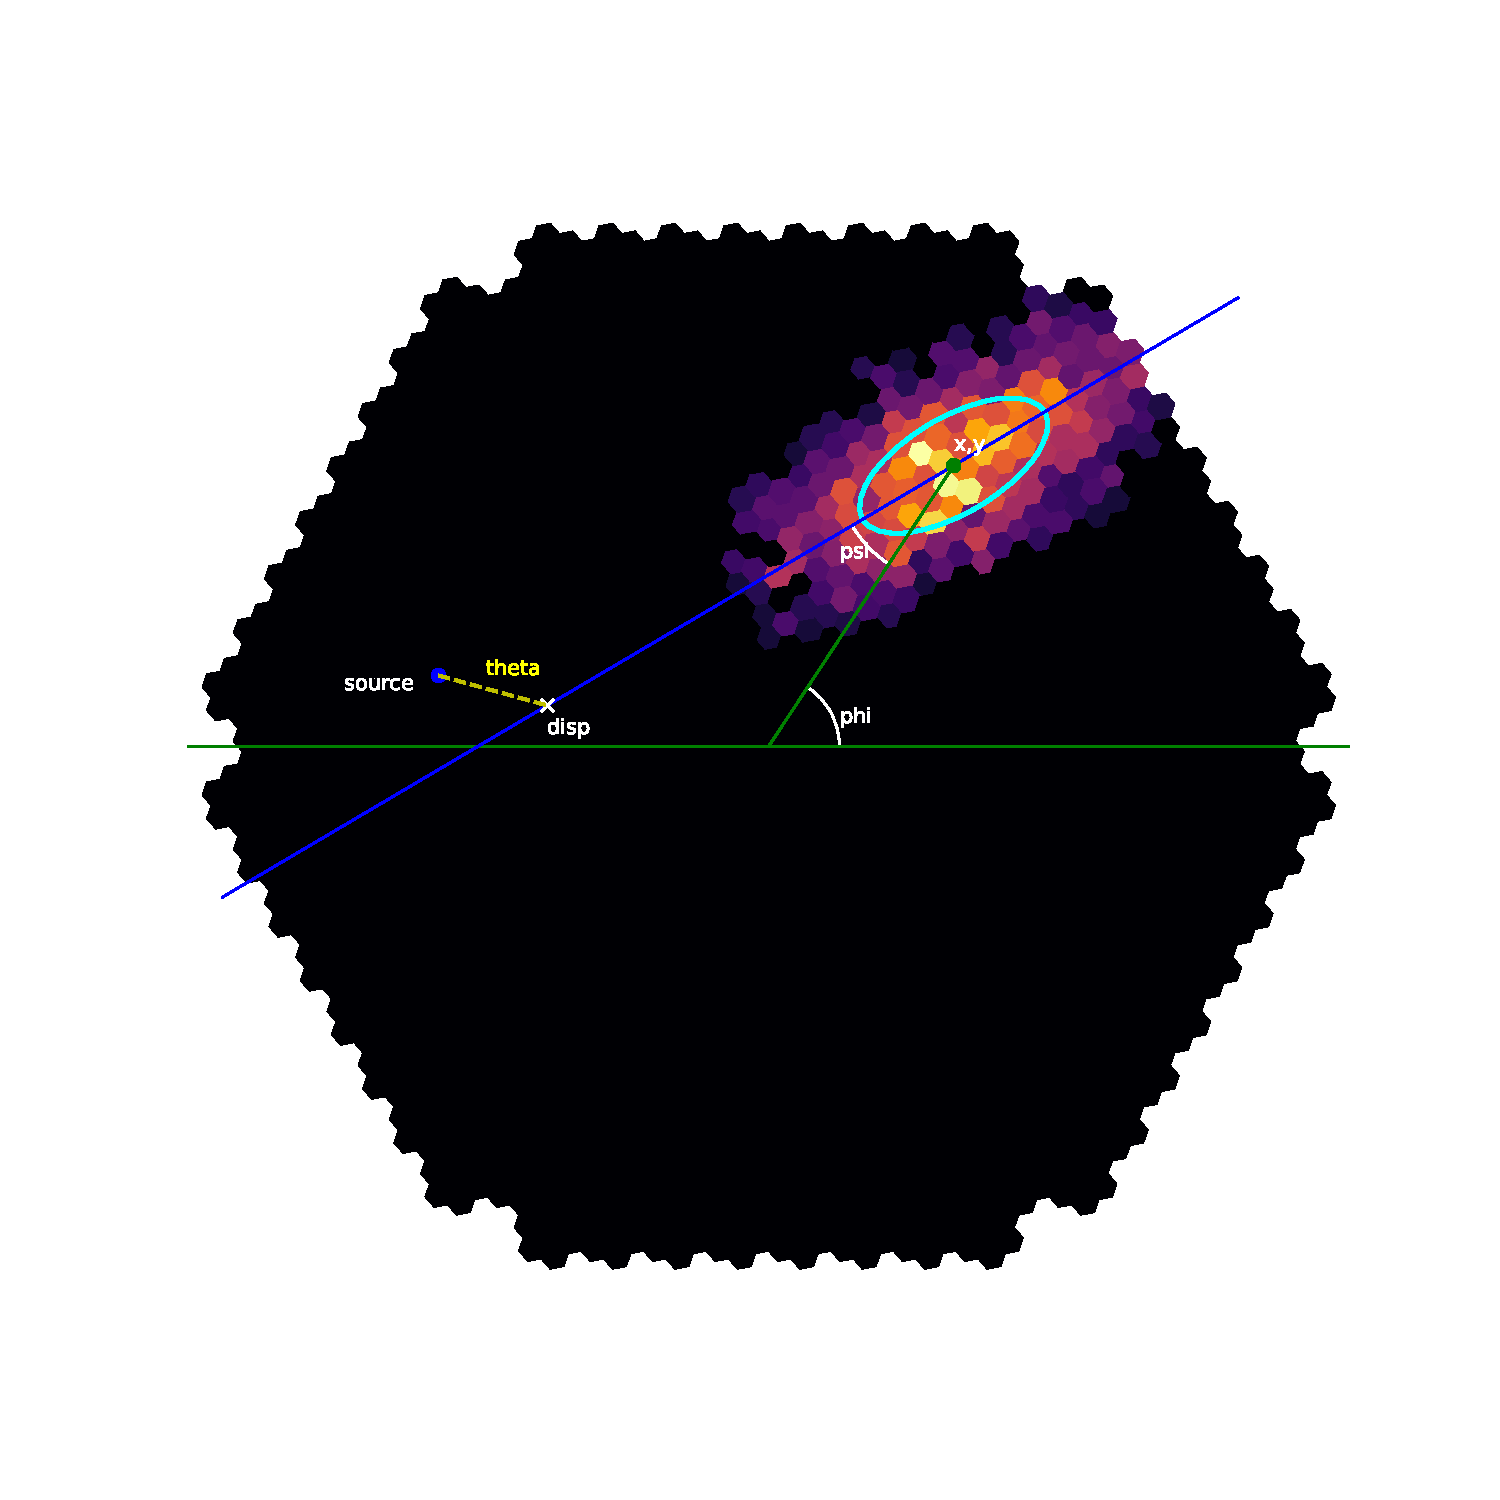
\includegraphics[width=.6\textwidth]{Plots/hillas_complete.pdf}
	\caption{The same cleaned shower-image as in figure \ref{fig:shower_cleaning}
	with the hillas-parameters calculated and marked in the camera frame.
	The parameters $\phi$, $\psi$, $x$ and $y$ describe the 
	orientation and position of the shower ellipse in the camera frame.
	The shower axis constrains the possible source position. 
	Applying the DISP-method two possible points remain.}
	\label{fig:hillas_params}
\end{figure}

With the hillas parameters calculated, the reconstruction of the 
primary particles properties can be done:

The primary \textbf{particle energy} is mostly described by the contained light in the image combined with 
an estimate of how much of the light missed the camera. 

The \textbf{particle type} can be reconstructed 
by looking at the image shape.
As we saw earlier, $\gamma$ and hadronic showers have different properties, 
resulting in different images. The assumption of a single, elliptic signal
area only works reasonably well for $\gamma$-showers.
A representation of different shower types can be seen in figure \ref{fig:compare_showers}.

\begin{figure}
	\centering
	\captionsetup{width=0.9\linewidth}
	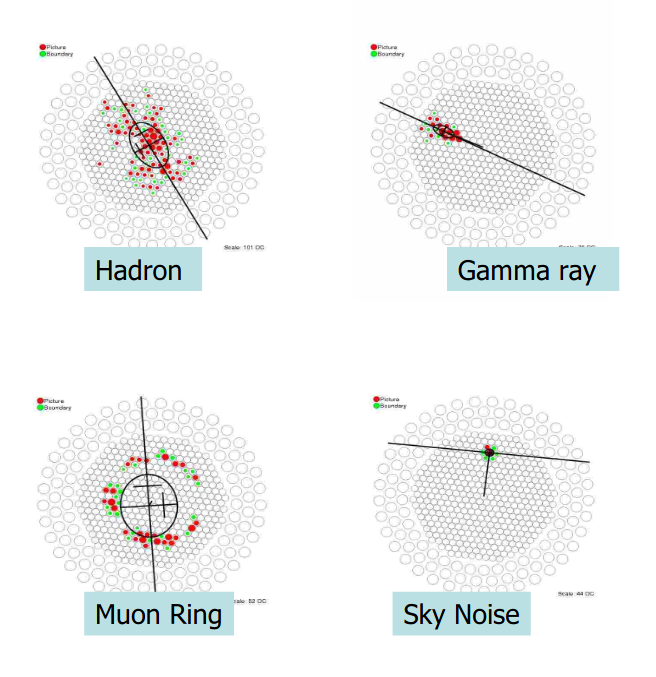
\includegraphics[width=.9\textwidth]{images/shower_types.png}
	\caption{A comparison of different shower types as seen 
	by the Whipple telescope.
	Hadronic showers are more separated than gamma showers and tend to
	form multiple clusters in the camera.
	Muons often times produce ring-like images in the camera (WHY?).
	The image is taken from an introduction lecture by Albrecht Karle \cite{icecube_showers}.}
	\label{fig:compare_showers}
\end{figure}

For the reconstruction of the \textbf{source position}
one possible way involves using the DISP-method in some way.

As basic estimation one can predict the shower origin by 
transforming the center of gravity (cog) of the image onto the sky plane.
The DISP-method assumes that the 
center of gravity is displaced relative to the
real source position depending on the angle the photon arrived at the telescope.
With higher angles the shower ellipse gets more eccentric as well.
The ellipsicity of the ellipse is thus a measure for the displacement of the true 
source position.
If one assumes the true source position to be on the main shower axis of the ellipse,
finding this position simplifies to finding a single point on the main shower axis.

Monoscopic experiments, that make use of the DISP method, need to resolve the head-tail-ambiguity:
Knowing the distance from the cog leaves two possible points, one on either side 
of the ellipse.
Stereoscopic experiments can resolve this ambiguity by combining the images from 
multiple telescopes, as can be seen in figure \ref{fig:stereo_shower}.

\begin{figure}
	\centering
	\captionsetup{width=0.9\linewidth}
	\hspace*{0.1\textwidth}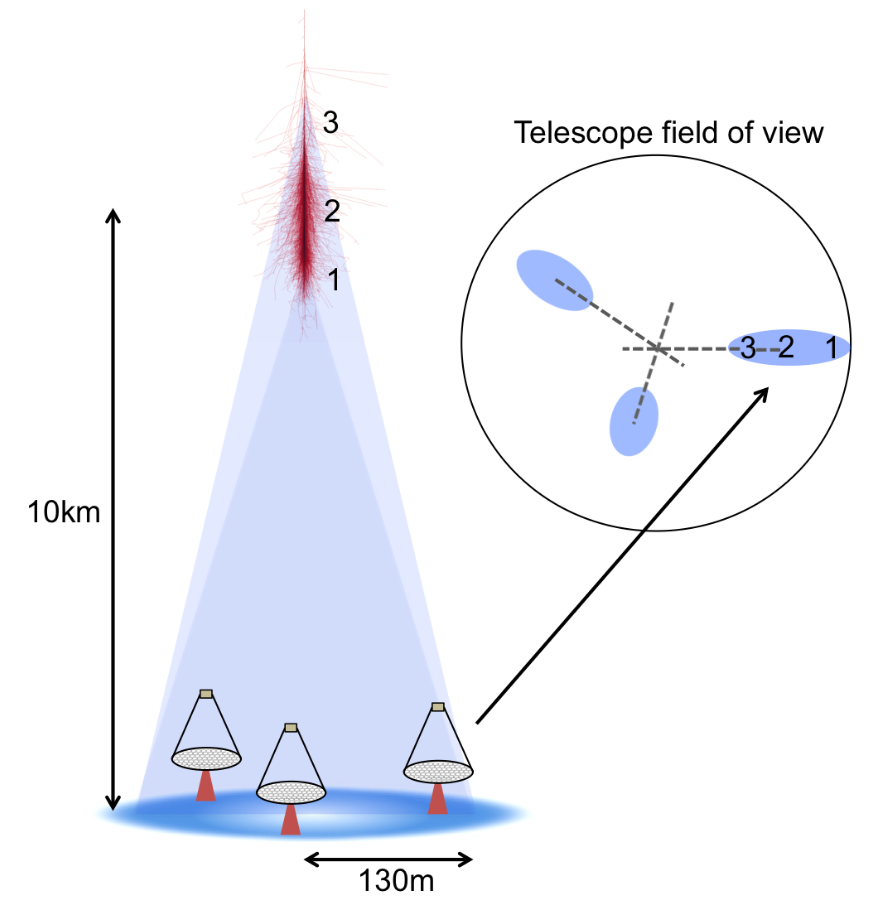
\includegraphics[width=0.9\textwidth]{images/stereo_shower.png}
	\caption{An illustration of an air shower captured with multiple telescopes.
		Each telescope captures an elliptic image.
		The image axes get intersected to reconstruct the arrival direction
		of the primary particle.
	    The image is taken from \cite{2015arXiv151005675H}.}
	\label{fig:stereo_shower}
\end{figure}



\chapter{Cherenkov Astronomy and CTA}
\label{cta}


\section{A Brief History of Ground Based Atmospheric Cherenkov Astronomy}
In the time between the discovery of cosmic radiation by Victor Hess
and today there have been various different attempts to investigate its origins.
Experiments have been conducted in various forms like Cherenkov telescopes, scintillator 
arrays and satellites.

To understand the motivation behind CTA, 
we will focus on the ground-based 
cherenkov telescopes and split our brief look at history 
into three generations as proposed by Turver and Weekes \cite{turver1980}.

During a Royal Society meeting in 1981 they presented ways to improve on
the so called first generation of telescopes by taking images of the shower
and exploiting stereoscopy with multiple telescopes, which are both central
concepts to modern experiments.

\subsection{The First Generation}
\label{sec:1stgen_iact}
The first generation of Cherenkov telescopes 
lacked any kind of imaging as is present in all of the bigger new experiments.
Instead they initially consisted of a single mirror with a single photo multiplier on top.
One of the earliest attempts to catch the cherenkov light emitted by cosmic rays 
was by Galbraith and Jelley in 1953 \cite{1953Natur.171..349G}, who found very few pulses
above background level with their experiment consisting of a very simple 
telescope and an array of Geiger-Müller counters used for coincidence measurements.

A more sophisticated approach was later taken with the Whipple telescope:
It consisted of 252 small mirrors providing a large detector area and operated between 
1968 and 1976. The multi-mirror design made it feasible to build the large 10m diameter 
mirror without exploding on the construction cost.
The telescope stayed operational for long after its primary observation time
when the Whipple collaboration eventually became the VERITAS collaboration 
and used the telescope to test new hardware and upgrades \cite{whipple1968}.


\subsection{The Second Generation}
To research the effectiveness of the "imaging approach", in 1982 the groups around Fegan and Weekes
installed an imager consisting of 37 photo multipliers at the no longer used Whipple telescope.
This later got replaced by a more capable 109-pixel camera that can be seen in figure \ref{fig:whipple_cam}.

\begin{figure}
	\centering
	\captionsetup{width=0.9\linewidth}
    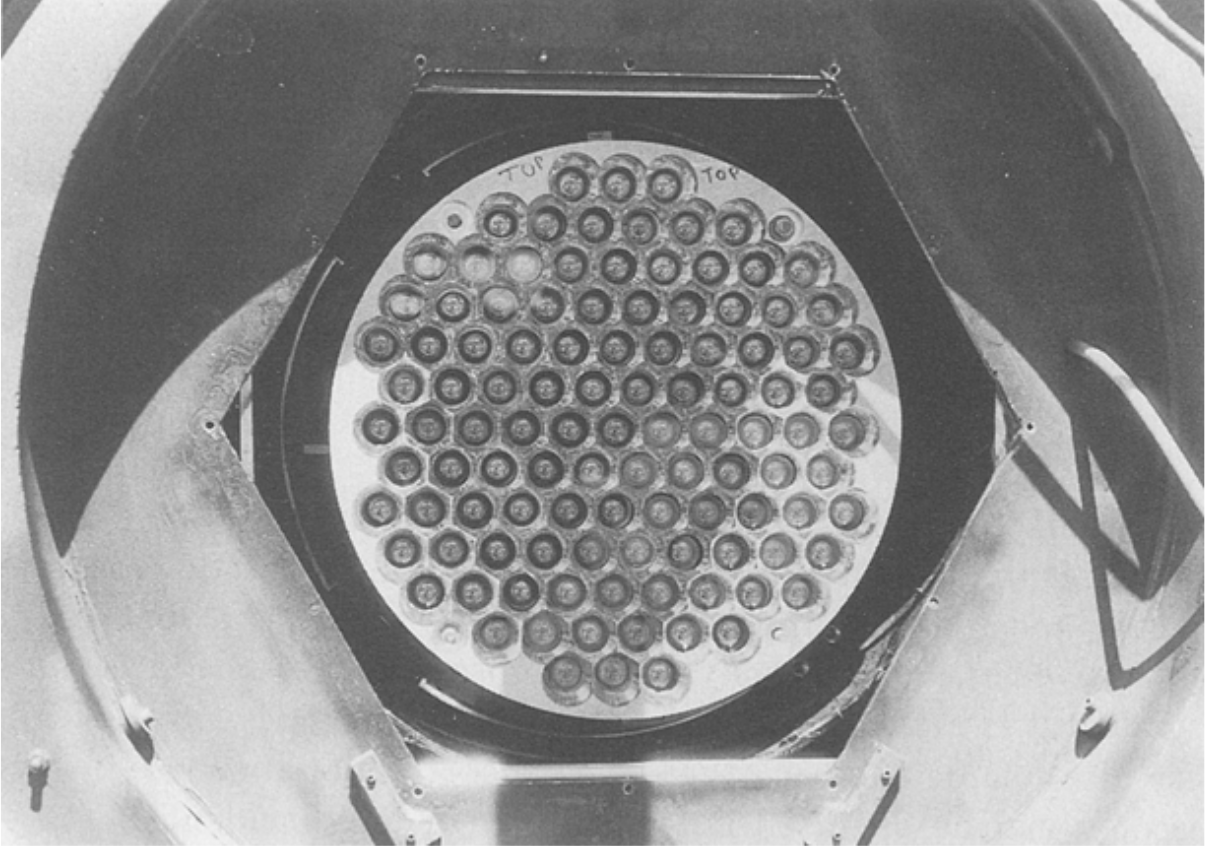
\includegraphics[width=0.5\textwidth]{images/whipple_cam.png}
    \caption{
		Picture of the upgraded camera of the Whipple telescope as it was in use in 1994.
		In this form it included 109 pixels, spaced at \SI{0.25}{\degree} \cite{Cawley1995}.}  % not the best source
    \label{fig:whipple_cam}
\end{figure}

The shower images in combination with better computer simulations allowed for 
superior background rejection based on the  hillas-parameters.
1989 had the telescope observing the Crab Nebula with 9$\sigma$ 
\cite{1989ApJ...342..379W}.

To improve on the sensitivity, a new method to reconstruct 
the arrival direction was tested in 2000 \cite{Lessard:2000yf}.
For this method a new parameter was defined, that describes a correction factor 
for the source position in the camera field relative to the center of gravity.
This method was further refined at the MAGIC-telescopes as the already mentioned DISP-method.

Another big experiment of the time was the HEGRA experiment, an array consisting 
of 37 \SI{1}{\meter^2} scintillation detectors \cite{ALLKOFER1990345} in the first stage.
Although at this stage not technically an IACT-experiment, later upgrade plans
brought multiple \SI{8.5}{\meter^2} diameter telescopes, starting with the first 
telescope in 1985 \cite{DAUM19971}.
While each telescope does not look too impressive on its own,
the so called HEGRA-IACT array made for a great use of the stereo principle,
marking the transition to the third generation of IACTs.


\subsection{The Third Generation}

Towards the end of the 1990s several third generation experiments were
proposed:
H.E.S.S and MAGIC, deriving from parts of the HEGRA collaboration, 
VERITAS from Whipple and the no longer operating CANGAROO from Adelaide and 
several japanese universities \cite{HILLAS201319}. All of these
were designed as stereoscopic imaging telescopes building on the progress made during the 
second generation with two experiments located on each the north and the south hemisphere.

\subsubsection{Major Atmospheric Gamma Imaging Telescopes (MAGIC)}
MAGIC is a experiment nowadays operating as a stereo setup of two telescopes.
Both telescopes are located at La Palma and have a \SI{17}{\meter} diameter mirror \cite{ALEKSIC201676}.

In the first phase MAGIC consisted of a single telescope, for differentiation usually
referred to as MAGIC-I, making MAGIC a second generation experiment. This first phase started 
operation in 2004 and had MAGIC-I be the largest IACT of its time.

The addition of MAGIC-2, the second mostly identical telescope, in 2012 marked the 
start of the second phase of the experiment and the transition to a third 
generation experiment \cite{2009arXiv0907.1211C}.
In the second phase MAGIC operates in the energy range from \SI{30}{\giga\eV}
up to \SI{100}{\TeV} \cite{magic_website}.

The DISP-method for the reconstruction of the event arrival direction 
was significantly improved by including timing information and showed better 
results for stereoscopy than the simple crossing of the main shower axis \cite{ALEKSIC2012435}.

A specialty of the MAGIC experiment lies in its ability to 
perform fast skews and thus react to gamma ray bursts after they have been observed 
by satellite experiments \cite{2003ICRC....5.2943B}.
This enabled the recent observation of the very first \si{\TeV}
gamma ray burst observed with IACTs \cite{collaboration2019teraelectronvolt}.


\subsubsection{Very Energetic Radiation Imaging Telescope Array System (VERITAS)}
VERITAS	was initially planned as a seven-telescope array, arranged in a diamond shape
\cite{WEEKES2002221}.

Eventually the collaboration settled 
with four telescopes. 
Each telescope covers a 3.5° FoV with a \SI{12}{\meter} diameter mirror and 
a 499 pixel PMT camera.

A relocation of telescope 1 in 2009 meant that the 
experiment made better use of the given area and its four telescopes,
improving the sensitivity by up to 30\% \cite{2009arXiv0912.3841P}.
The old and new layout can be seen in figure \ref{fig:veritas_relocation}.

The VERITAS collaboration mentions a lower threshold of \SI{100}{\giga\electronvolt}
with the four telescope setup.

\begin{figure}
	\center
	\captionsetup{width=0.9\linewidth}
	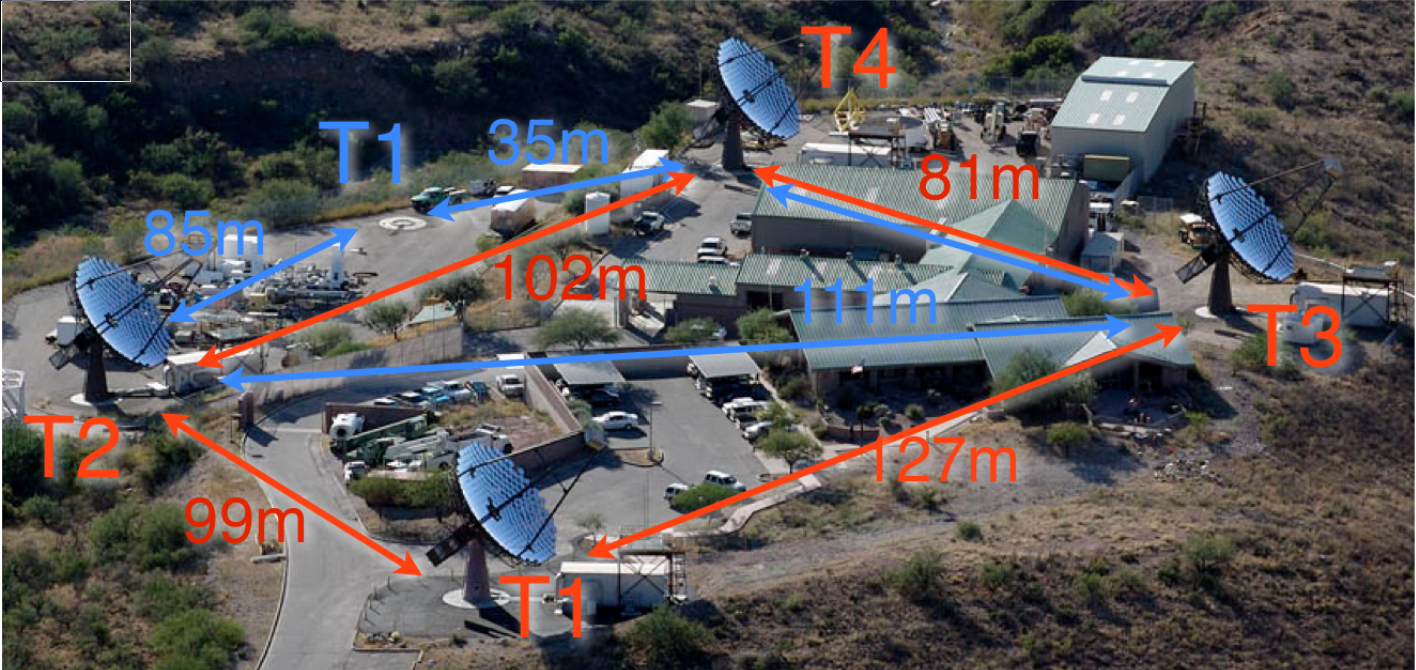
\includegraphics[width=.9\textwidth]{images/veritas_relocation.png}
	\caption{The VERITAS array layout after relocation of the first 
		telescope. The distances between the telescopes are 
		highlighted for the old(blue) and the new(red) array.
		In the old setup the telescopes T1, T2 and T3 were too closely
		located, making their measurements redundant.
	 	The image is taken from an official paper, that investigates
		the improved performance gained by relocating the telescope \cite{2009arXiv0912.3841P}.}
	\label{fig:veritas_relocation}
\end{figure}

Like MAGIC, VERITAS makes use of the DISP-method, especially at large zenith angles 
\cite{2015ICRC...34..771P}.

\subsubsection{High Energy Stereoscopic System (HESS)}

The HESS experiment consists of five telescopes and 
is - in contrast to MAGIC and VERITAS - operating in the southern 
Hemisphere, in Namibia.

A similar distinction in phase I and phase II as with MAGIC can be taken with 
HESS phase I consisting of four \SI{13}{\meter} diameter telescopes,
arranged at the edge of a square of \SI{120}{\meter} long sides \cite{HINTON2004331}.
These operated from 2004 to 2012 when the experiment went into phase II.

Phase II brought the larger, fifth telescope with the aim to lower the energy threshold
further. This $\SI{24}{\meter} \times \SI{32}{\meter}$-mirror telescope 
was placed in the middle of the other telescopes.
HESS operates at a similar energy range as MAGIC, stating a lower threshold as low as 
\SI{20}{\giga\electronvolt} \cite{vincent2005hess}.


\section{Next to come: The Cherenkov Telescope Array (CTA)}
\label{sec:cta}

The Cherenkov Telescope Array aims to be a next generation IACT experiment.
With two sites of operation, one for each hemisphere, and a number of different 
telescopes proposed, CTA is going to expand on the findings of the third 
generation experiments.

Like HESS in phase II, the CTA arrays are going to consist of different sized telescopes, namely
the Large Sized Telescope (LST, \SI{23}{\meter}), 
the Medium Sized Telescope (MST, \SI{12}{\meter}) 
and the Small Sized Telescope (SST, \SI{4.3}{\meter}).

Extensive Monte Carlo simulations have been performed to find optimal array arrangements
\cite{BERNLOHR2013171}.

The currently planned layouts at LaPalma and in Chile are shown in 
\ref{fig:cta_layout}

\begin{figure}
	\center
	\captionsetup{width=0.9\linewidth}
	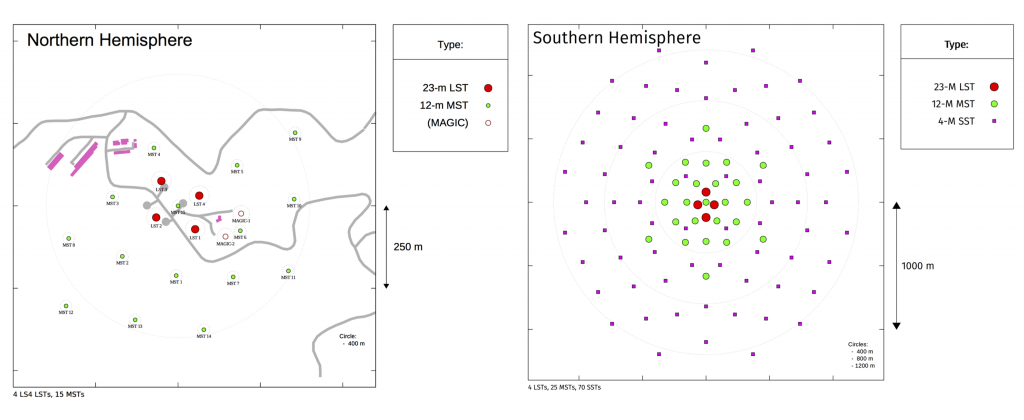
\includegraphics[width=0.9\textwidth]{images/cta_layout.png}
	\caption{The planned layouts for CTA. The dots mark the telescope types.
	Left: The array on the northern hemisphere. It will be build at LaPalma
	and feature only LSTs and MSTs.
	Right: The array at the southern hemisphere.
	It will consist of more telescopes and thus 
	work at a bigger energy range.
	\cite{cta_web}}
	\label{fig:cta_layout}
\end{figure}


\subsection{LST}
\label{sec:lst}

The Large-Sized Telescope is going to be biggest telescope of CTA
with a mirror diameter of \SI{23}{\meter}.
It will provide the best sensitivity in the energy range from 
\SI{20}{\giga\electronvolt} to \SI{150}{\giga\electronvolt} with a field of view of \SI{4.3}{\degree}.
The camera of the LST, the LSTCamera, has \num{1855} channels 
with \num{265} photomultiplier tubes \cite{cta_web}.
The readout electronic is based on the Domino Ring Sampler 
Version 4 chip, which is also used by the MAGIC experiment
\cite{Kubo:2013pwa}. 

Since the LST is looking for the lowest energy $\gamma$-rays, it needs
very large mirror areas. At the same time the effective detector area does 
not need to be as high as for higher energy events.
For this reason only 4 telescopes are planned per array.

The first LST has been inaugurated at the 10 October 2018 in La Palma \cite{lst_debut}.

\begin{figure}
	\center
	\captionsetup{width=0.9\linewidth}
	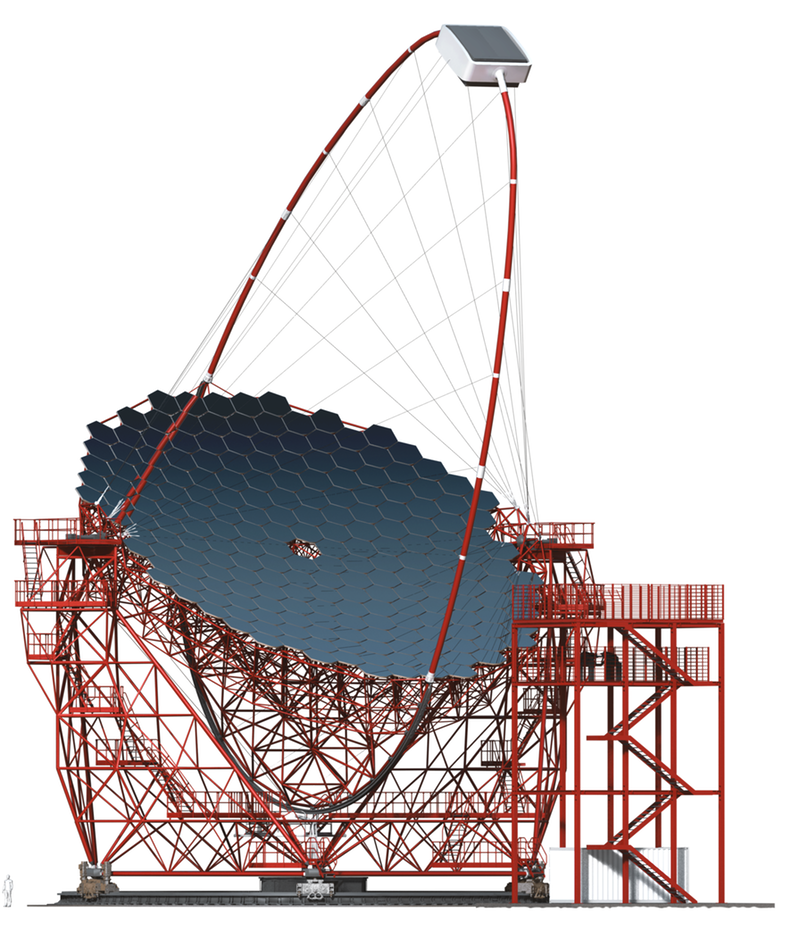
\includegraphics[width=.4\textwidth]{images/LST.png}
	\caption{
		An illustration of the Large Sized Telescope (LST) with its
		\SI{23}{\meter} diameter parabolic mirror.
		In the lower left corner a human is included for scale.
		The image can be found at the official CTA-website \cite{cta_web}.}
	\label{fig:lst}
\end{figure}

\subsection{MST}

The Medium-Sized Telescopes (MST) are primarily going to look at the 
energy range from \SI{150}{\giga\electronvolt} to \SI{5}{\tera\electronvolt}.
A total of 15 telescopes on the north site and 25 telescopes at the south site 
are going to be the backbones of CTA.
Two camera designs are being tested for the MST:
The 1764 pixel FlashCam and the 1855 pixel NectarCam \cite{cta_web}.

\begin{figure}
	\center
	\captionsetup{width=0.9\linewidth}
	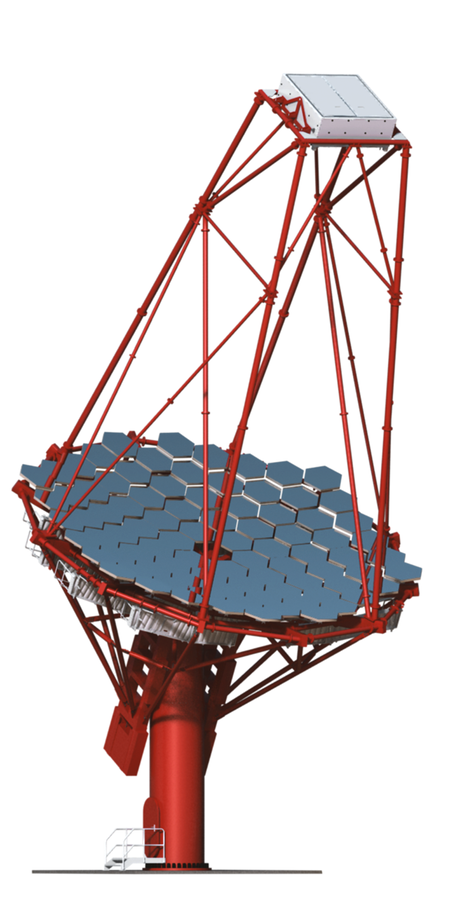
\includegraphics[width=.4\textwidth]{images/MST-1.png}
	\caption{An illustration of the Mid Sized Telescope (MST) with its
	\SI{11.5}{\meter} diameter mirror.
	The mirror design is based on the Davies-Cotton design.
	The image can be found at the official CTA-website \cite{cta_web}.}
	\label{fig:mst}
\end{figure}



\subsection{SST}
The Small-Sized Telescopes (SST) will provide the sensitivity for CTA at the 
highest energies upwards from \SI{5}{\tera\electronvolt}.
An upper limit for the sensitivity is expected to be around \SI{300}{\tera\electronvolt}.

The design for the SST includes two mirrors, a \SI{4.3}{\meter} and a \SI{1.8}{\meter}
mirror, before the light hits the camera.

In contrast to the LST and MST, the SST's camera includes silicon photo-multipliers
and a total of 2368 pixels. With this the SST is going to cover a field of view 
of \SI{10.5}{\degree}.

The north array is not going to include any SSTs, the 
south array on the other hand will contain a total of 70 telescopes over
several square kilometers \cite{cta_web}.

\begin{figure}
	\center
	\captionsetup{width=0.9\linewidth}
	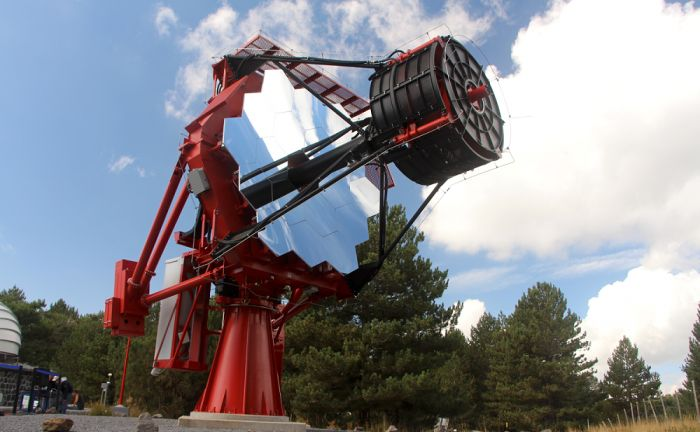
\includegraphics[width=.9\textwidth]{images/sst.jpg}
	\caption{An illustration of the Small Sized Telescope (SST) with its
	two mirrors.
	The dual-mirror Schwarzschild-Couder setup includes mirrors of
	\SI{4.3}{\meter} and \SI{1.8}{\meter} diameter.
	The image can be found at the official CTA-website \cite{cta_web}.}
	\label{fig:sst}
\end{figure}


\chapter{Machine Learning Basics}
\label{ml}

CTA, much like every other big experiment in (astro-)particle physics,
is going to produce enormous amounts of data.
Depending on the number of installed telescopes, multiple
\si{\peta\byte} per year are expected to be saved
on disk and tape \cite{lamanna2015cherenkov}.

Given these enormous amounts of data, it comes as no surprise that
various data reduction techniques need to get applied in
order to reduce data size.
Multiple machine learning models have proven to be
quite successful in solving classification and
regression problems
\cite{bigdata_astronomy}.

This thesis focuses on using random forests to
perform the gamma/hadron separation
and estimation of the source position.
To understand how these algorithms work, we will
have a short look into some basics
of the necessary machine learning concepts.

\section{Supervised learning}
In the task of supervised machine learning a model is trained on a
dataset with full information available.
This data will come from Monte Carlo simulations in our case, but
could also be e.g. historical or hand labeled datasets in other contexts.
The trained model can then later be used to estimate features on a dataset, which
lacks the needed information.

We define a dataset as having a number of samples with a fixed number of
variables (features) each.
In the following we split
the features of our dataset into a set of \textbf{input} variables $X$ and
a set of \textbf{output} variables $y$.

The naming convention for
these sets follows the one of scikit-learn
\cite{scikit-learn}, \cite{sklearn_api}, a python package for
machine learning algorithm.
We will later use scikit-learn as a basis to train our machine learning models.
Other terminologies for the two feature sets include
predictors or independent variables for the input, and
responses or dependent variables for the output.


\section{Classification}
In (supervised) classification tasks, we want to predict of which of some
predefined classes the given sample is a member. The possible solutions for $y$
are from a discrete set of values in
contrast to a regression problem with a continuous solution space.
A model that performs classification on data is referred to as a
classifier.

The simplest and most popular case of classification problems
is \textbf{binary classification} \cite{sokolova2009systematic}.
In this case only two distinct
classes exist, which fortunately is all we will need for
our signal/background-separation.
A common example for a classification problem is an Email spam filter,
where mails get categorized in at least two categories based
on their content and meta data \cite{DBLP:journals/corr/cs-CL-0006013}.

For binary classification we can define a set of measures
to define the quality of our prediction, starting with the confusion matrix
shown in table \ref{tab:confusion},
with $pos$ referring to the true label of the positive (i.e. signal)
and $neg$ referring to the label of the negative (i.e. background) class.

\begin{table}
    \caption{Definition of a confusion matrix for binary classification.
    The main diagonal includes the correct predictions, wrong predictions are on the off diagonal.}
    \begin{center}
        \begin{tabular}{ l| l l}
            %\hline
            {} & Predicted as $pos$ & Predicted as $neg$ \\
            \hline
            $pos$ & true positive ($tp$) & false negative ($fn$) \\
            %\hline
            $neg$ & false positive ($fp$) & true negative ($tn$) \\
            %\hline
        \end{tabular}
    \end{center}
    \label{tab:confusion}
\end{table}

An ideal classification would result in
\begin{equation*}
  fp = fn = 0.
\end{equation*}

Based on the confusion matrix, multiple measures
can be constructed to examine the classifiers performance.
Some of the more common ones are listed in table \ref{tab:class_metrics}.

\begin{table}
    \caption{Popular metrics for binary classification tasks.}
    \begin{center}
        %\caption{
         % Common metrics for classification tasks, taken from \cite{sokolova2009systematic}.}
        \begin{tabularx}{\textwidth}{l c X}
            %\hline
            Measure & Formula & Interpretation \\
            \hline
            Accuracy & $\frac{tp+tn}{tp+fn+fp+tn}$ & Overall effectiveness of a classifier \\
            %\hline
            Precision & $\frac{tp}{tp+fp}$ & Class agreement with the positive labels given by the classifier \\
            %\hline
            Recall/Sensitivity & $\frac{tp}{tp+fn}$ & Effectiveness of a classifier to identify positive labels \\
            %\hline
            F$_{\beta}$-score & $\frac{(\beta^2+1)tp}{(\beta^2+1)tp+\beta^2fn+fp}$ & Harmonic mean between precision and recall with choosable $\beta$ \\
            %\hline
            Specificity & $\frac{tn}{fp+tn}$ & How effectively a classifier identifies negative labels \\
            %\hline
            Balanced Accuracy & $\frac{1}{2}(\frac{tp}{tp+fn}+\frac{tn}{fp+tn})$ & Classifier’s ability to avoid false classification \\
        %\hline
        \end{tabularx}
        %\caption{Overview of common metrics for classification tasks based on the
        %intermediate metrics shown in table \ref{tab:confusion}}
    \end{center}
    \label{tab:class_metrics}
\end{table}

We will make use of the precision, recall and F-score.
Additionally we will calculate the Area Under the Curve (AUC) with regard to the Receiver Operating Characteristic (ROC) curve.
The ROC-curve is gained by plotting the true positive rate against the false positive rate while varying the classifier threshold.
The area under the (normalised) ROC-curve is thus a measure for whether the classifier will
rank a randomly chosen positive sample higher than a randomly chosen negative sample \cite{FAWCETT2006861}.

\section{Regression}
Regression is the task of predicting a continuous variable
from a set of input variables.
The simplest approach
to this problem is the ordinary linear least squares method.

Given an unrestricted linear model
\begin{align}
	y &= X\beta + e \\
	E(y) &= X\beta \\
	Cov(y) &= \sigma^2 I_n
\end{align}
with a measured vector $y$, the design matrix $X$,
an unknown parameter vector $\beta$, a random error $e$
and pairwise orthogonal features $y_i$,
the least-squares solution is given by the solution of
the minimizing problem in equation \ref{eq:min_least_squares}.

\begin{equation}
	\min_{\beta\in\mathbb{R}^k} \lVert y - X\beta \rVert
	\label{eq:min_least_squares}
\end{equation}

If $(X^TX)^{-1}$ exists, the unique solution for the
least square estimation of $\beta$ becomes:
\begin{equation}
	\hat{\beta} = X^+ y,
\end{equation}

with the Moore-Penrose inverse $X^+ = (X^TX)^{-1}X^T$.
The estimation of $y$ then becomes:
\begin{equation}
  \hat{y} = X\hat{\beta}.
\end{equation}

The metric, that is minimized by the least-squares solution
is the Mean Squared Error (MSE).

Other metrics for regression tasks include the
Root-Mean-Squared-Error(RMSE),
Mean-Absolute-Error(MAE)
or the Coefficient of Determination ($R^2$), all of which are listed in table
\ref{tab:regr_metrics}.

\begin{table}
  \caption{Popular metrics for a regression problem with $n$ samples.}
  \begin{center}
    \begin{tabularx}{\textwidth}{l c X}
      Measure & Formula & Interpretation \\
      \hline
      Mean squared error & $\frac{1}{n}\sum_i^n |y_i-\hat{y_i}|$ & Prediction error disregarding the direction of over- and underprediction \\
      Mean absolute error & $\frac{1}{n}\sum_i^n (y_i-\hat{y_i})^2$ & For an unbiased predictor: Variance of the regressor. Heavily weights outliers. \\
      Coefficent of Determination & $1 - \frac{\sum_i^n (\bar{y_i}-\bar{y})^2}{\sum_i^n (y_i-\bar{y})^2}$ & Share of observed variance that is explained by the model.\\
    \end{tabularx}
  \end{center}
  \label{tab:regr_metrics}
\end{table}

Many metrics closely connected to these metrics exist, such as root mean squared error (RMSE)
or the mean absolute percentage error (MAPE).
Our analysis will be based on the use of the MSE.

\iffalse
% nicht mehr nötig, da keine Energieregression?
\subsection{Bias and Variance}
Bias und Varianz erklären!
\fi

\section{Decision Trees and Random Forests}
Methods based on Decision Trees work by recursively partitioning
the parameter space until the remaining samples behave similar enough.
Tree-based methods can be applied to both classification and regression tasks.

Forest methods combine multiple tree predictors to get more stable
predictions.

\subsection{Decision trees}
A simple (binary) decision tree
for an example classification on the iris dataset
is shown in figure \ref{fig:03_tree}.

\begin{figure}
  \centering
  \captionsetup{width=0.9\linewidth}
  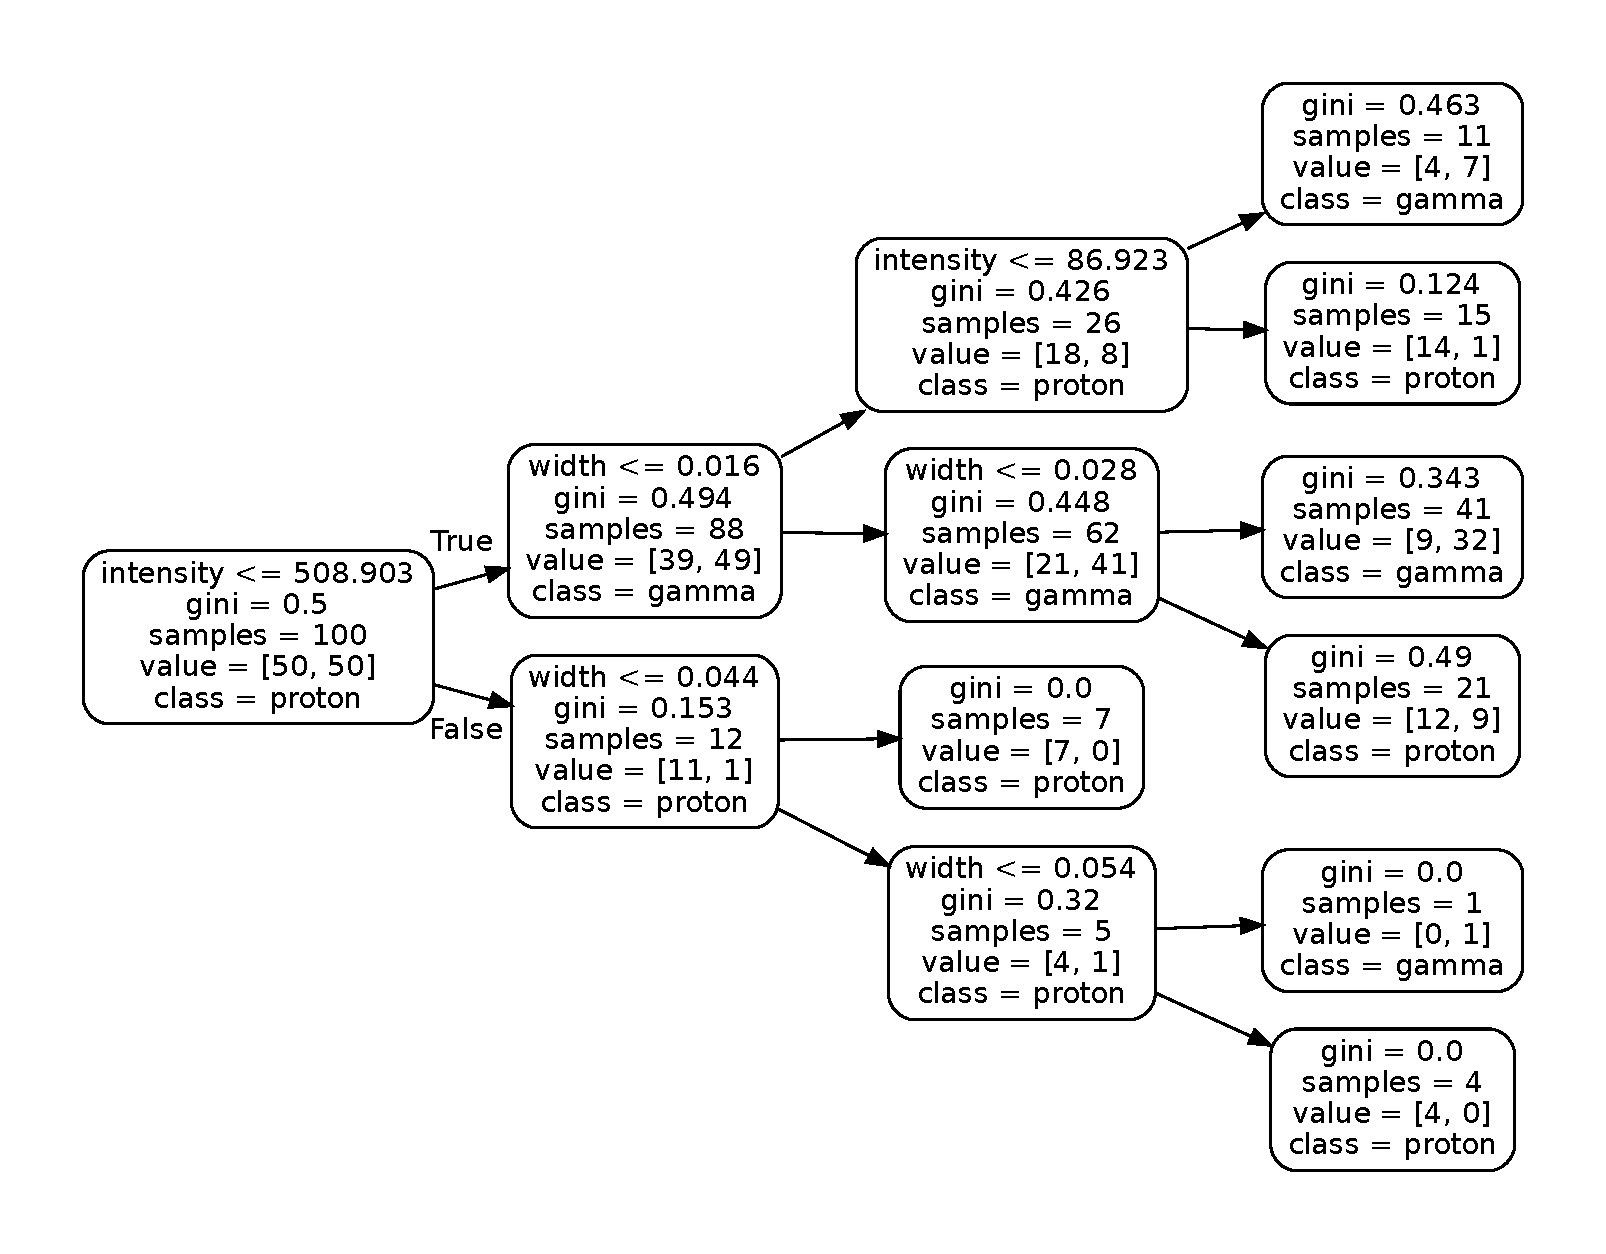
\includegraphics[width=0.9\textwidth]{Plots/decision_tree.pdf}
  \caption{A very simple decision tree for demonstrational purposes.
      The dataset in use is the famous iris dataset that includes
      measurements of the petal and sepal width and length
      for three different flower classes \cite{fisher1936use}.
      Each node lists (from top to bottom): The cut that will
      be applied with the samples fulfilling the condition going
      into the left node and the remaining samples in the right node.
      The gini coefficient evaluated on the associated samples.
      Once it reaches zero, no further splits are performed.
      The number of samples that ended up in the node and last the
      class distribution in the samples.
      One can derive that the first class can immediately be separated from
      the other two classes (left node, first split), while the other two classes
      are harder to separate and require multiple cuts for a perfect separation.}
  \label{fig:03_tree}
\end{figure}

Starting from the root node, a binary split is performed to
split up the data. For each resulting node additional splits are performed
until a stopping criterion is reached.
Choosing the optimal split is defined as minimizing a
pre-defined measure.

For classification tasks this means reducing the class impurity in the node.
Often used measures
to quantify the impurity are gini coefficient, that is used in the example, or the
cross-entropy \cite{hastie2017springer}.
Both are defined in equation \ref{eq:gini_ce}

\begin{align}
	\text{Gini impurity: } &= \sum_{k=1}^K \hat{p}_{mk}(1-\hat{p}_{mk}) \\
	\text{Cross-entropy: } &= -\sum_{k=1}^K \hat{p}_{mk}\log{\hat{p}_{mk}},
  \label{eq:gini_ce}
\end{align}

with $p_{mk}$ denoting the proportion of class $k$ in node $m$.

A stopping criterion can be defined as the measure reaching a
a defined threshold or not improving anymore.
Alternatively the tree can stop at a predefined depth to
avoid overly complex models.

For regression tasks scikit-learn uses the mean squared error
or mean absolute error and the same principles apply.
We will later use the Gini impurity and the Mean Squared Error
for the classification and regression tasks respectively.

The implementation in sklearn is based on the one by
Leo Breiman et al \cite{breimanclassification}.
A single tree performs binary splits $\Theta = (j, t_m)$
at each node $m$ in order to split
the data at this node $Q$ into two subsets
$Q_\text{left}$
and
$Q_\text{right}$.
The split consists of a feature $j$ and a threshold $t_m$ and is
chosen in a way to minimize the given measure.
Features, that are more important for the task, will
thus appear at the top nodes of the tree.


While decision trees have the benefit of providing
easily interpretable, low bias models there are some drawbacks to this
approach, namely \cite{hastie2017springer}:
\begin{itemize}
  \item{Instability, high variance}
  \item{Lack of Smoothness}
  \item{Difficulty in Capturing Additive Structure}.
\end{itemize}

Approaches to reducing these problems include
boosting \cite{freund1997decision} and Random Forests \cite{Breiman2001}.

\subsection{Random Forests}

Random forests have become one of the standard algorithms
in data analysis tasks, because according to our
experience and \cite{hastie2017springer} they tend to
rarely overfit (as long as the individual trees have no or little bias)
and generally perform decent without a lot of manual tuning.

The main idea behind random forests is to use multiple, independent
decision trees to suppress the problems single trees have, while
keeping their advantages.
For this to work, the individual trees need not to be correlated.
Consequently the trees cannot all be constructed the same way.
To make sure the individual trees
- and their predictions -
are somewhat independent from each other,
some kind of randomness has to be introduced to the tree.
In random forests this is on the one hand achieved by giving each tree a
randomly drawn subsample from the training data.
This is referred to as bootstrapping \cite{efron1992bootstrap}.
Another source of randomness is to perform splits on a node
based on only a random subsample of the available features.

The prediction of the random forest in scikit learn is then the average of
the single trees predictions.
In the case of a classification task, the probabilistic predictions for each class
get averaged.

\iffalse
\section{mean estimation stuff, outlier resistance, unsupervised? clusters?}
warum robuste schätzer?
verwendete algorithmen
\fi

